%%
%% Copyright 2007, 2008, 2009 Elsevier Ltd
%%
%% This file is part of the 'Elsarticle Bundle'.
%% ---------------------------------------------
%%
%% It may be distributed under the conditions of the LaTeX Project Public
%% License, either version 1.2 of this license or (at your option) any
%% later version.  The latest version of this license is in
%%    http://www.latex-project.org/lppl.txt
%% and version 1.2 or later is part of all distributions of LaTeX
%% version 1999/12/01 or later.
%%
%% The list of all files belonging to the 'Elsarticle Bundle' is
%% given in the file `manifest.txt'.
%%

%% Template article for Elsevier's document class `elsarticle'
%% with numbered style bibliographic references
%% SP 2008/03/01
%%
%%
%%
%% $Id: elsarticle-template-num.tex 4 2009-10-24 08:22:58Z rishi $
%%
%%
\documentclass[preprint,12pt,3p]{elsarticle}

\usepackage{color}
\usepackage{listings}
\usepackage{algorithm}
\usepackage{algorithmic}
\usepackage{amsmath}
\usepackage{subfigure}
\usepackage{xspace}
\usepackage[colorlinks,bookmarksopen,bookmarksnumbered,citecolor=red,urlcolor=red]{hyperref}

\newcommand{\DSVMP}{\textsc{Dsvmp}\xspace}
\newcommand{\tabincell}[2]{\begin{tabular}{@{}#1@{}}#2\end{tabular}}
\newcommand\FIXME[1]{\textcolor{red}{FIX:}\textcolor{red}{#1}}
\lstdefinelanguage
   [x64]{Assembler}     % add a "x64" dialect of Assembler
   [x86masm]{Assembler} % based on the "x86masm" dialect
   % with these extra keywords:
   {morekeywords={CDQE,CQO,CMPSQ,CMPXCHG16B,JRCXZ,LODSQ,MOVSXD, %
                  POPFQ,PUSHFQ,SCASQ,STOSQ,IRETQ,RDTSCP,SWAPGS, %
                  rax,rdx,rcx,rbx,rsi,rdi,rsp,rbp, %
                  r8,r8d,r8w,r8b,r9,r9d,r9w,r9b}} % etc
\lstset{language=[x64]Assembler}

\definecolor{codegreen}{rgb}{0,0.6,0}
\definecolor{codegray}{rgb}{0.5,0.5,0.5}
\definecolor{codepurple}{rgb}{0.58,0,0.82}
\definecolor{backcolour}{rgb}{0.95,0.95,0.92}

\lstdefinestyle{mystyle}{
    backgroundcolor=\color{backcolour},
    commentstyle=\color{codegreen},
    keywordstyle=\color{magenta},
    numberstyle=\tiny\color{codegray},
    stringstyle=\color{codepurple},
    basicstyle=\footnotesize,
    breakatwhitespace=false,
    breaklines=true,
    captionpos=b,
    keepspaces=true,
    numbers=left,
    numbersep=5pt,
    showspaces=false,
    showstringspaces=false,
    showtabs=false,
    tabsize=2
}
\lstset{style=mystyle}

%% Use the option review to obtain double line spacing
%% \documentclass[preprint,review,12pt]{elsarticle}

%% Use the options 1p,twocolumn; 3p; 3p,twocolumn; 5p; or 5p,twocolumn
%% for a journal layout:
%% \documentclass[final,1p,times]{elsarticle}
%% \documentclass[final,1p,times,twocolumn]{elsarticle}
%% \documentclass[final,3p,times]{elsarticle}
%% \documentclass[final,3p,times,twocolumn]{elsarticle}
%% \documentclass[final,5p,times]{elsarticle}
%% \documentclass[final,5p,times,twocolumn]{elsarticle}

%% if you use PostScript figures in your article
%% use the graphics package for simple commands
%% \usepackage{graphics}
%% or use the graphicx package for more complicated commands
%% \usepackage{graphicx}
%% or use the epsfig package if you prefer to use the old commands
%% \usepackage{epsfig}

%% The amssymb package provides various useful mathematical symbols
\usepackage{amssymb}
%% The amsthm package provides extended theorem environments
%% \usepackage{amsthm}

%% The lineno packages adds line numbers. Start line numbering with
%% \begin{linenumbers}, end it with \end{linenumbers}. Or switch it on
%% for the whole article with \linenumbers after \end{frontmatter}.
%% \usepackage{lineno}

%% natbib.sty is loaded by default. However, natbib options can be
%% provided with \biboptions{...} command. Following options are
%% valid:

%%   round  -  round parentheses are used (default)
%%   square -  square brackets are used   [option]
%%   curly  -  curly braces are used      {option}
%%   angle  -  angle brackets are used    <option>
%%   semicolon  -  multiple citations separated by semi-colon
%%   colon  - same as semicolon, an earlier confusion
%%   comma  -  separated by comma
%%   numbers-  selects numerical citations
%%   super  -  numerical citations as superscripts
%%   sort   -  sorts multiple citations according to order in ref. list
%%   sort&compress   -  like sort, but also compresses numerical citations
%%   compress - compresses without sorting
%%
%% \biboptions{comma,round}

% \biboptions{}


\journal{Computers \& Security}

\begin{document}

\begin{frontmatter}

\title{
Enhance Virtual-Machine-Based Code Obfuscation Security through Dynamic Bytecode Scheduling
\footnote{
Extension of Conference Paper: a preliminary version of this article entitled ``Exploiting Dynamic Scheduling for VM-Based Code Obfuscation" by K. Kuang et el. appeared in the 15th IEEE International Conference on Trust, Security and
Privacy in Computing and Communications(TrustCom), 2016~\cite{kuang2016exploiting}. The extended version makes the following additional contributions over the conference paper: (1) it provides a more detailed description of the background and threat model (Section~\ref{sec:bak} and~\ref{sec:attack}); (2) it describes how the virtual interpreter dynamically changes the execution path at runtime using an algorithmic model (Section~\ref{sec:mvm-2} and Algorithm~\ref{Alg:VMcore-work}); (3) it provides new experimental results to evaluate the overhead of the proposed technique, providing new insights of the approach (Section~\ref{sec:benchmarktest}); (4) it adds a new experiment to evaluate the diversity of the protected structure at runtime (Section~\ref{sec:s-d}); (5) it includes new results to compare the proposed approach against two commercial VM protection systems, Code Virtualizer and VMProtect (Section~\ref{sec:comparetest}).
}
}
%\tnotetext[label0]{This is only an example}

%\author[label1,label2]{Author One\corref{cor1}\fnref{label3}}
\author[label1]{Kaiyuan Kuang}
\address[label1]{School of Information Science and Technology, Northwest University, China.}
\address[label2]{School of Computing and Communications, Lancaster University, UK}%\fnref{label4}}

\cortext[cor1]{Corresponding author. Email address: zytang@nwu.edu.cn}

\ead{kky@stumail.nwu.edu.cn}


\author[label1]{Zhanyong Tang\corref{cor1}}
\ead{zytang@nwu.edu.cn}

\author[label1]{Dingyi Fang}
\ead{dyf@nwu.edu.cn}

\author[label1]{Xiaojiang Chen}
\ead{xjchen@nwu.edu.cn}

\author[label2]{Zheng Wang}
\ead{z.wang@lancaster.ac.uk}

\begin{abstract}
Code virtualization built upon virtual machine (VM) technologies is emerging as a viable method for implementing code obfuscation to protect programs against unauthorized analysis. State-of-the-art VM-based protection approaches use a fixed scheduling structure where the program follows a single, static execution path for the same input. Such approaches, however, are vulnerable to certain scenarios where the attacker can reuse knowledge extracted from previously seen software to crack applications using similar protection schemes. This paper presents \DSVMP, a novel VM-based code obfuscation approach for software protection. \DSVMP brings together two techniques to provide stronger code protection than prior VM-based schemes. Firstly, it uses a dynamic instruction scheduler to randomly direct the program to execute different paths without violating the correctness across different runs. By randomly choosing the program execution paths, the application exposes diverse behavior, making it much more difficult for an attacker to reuse the knowledge collected from previous runs or similar applications to perform attacks. Secondly, it employs multiple VMs to further obfuscate the relationship between VM bytecode and their interpreters, making code analysis even harder. We have implemented \DSVMP in a prototype system and evaluated it using a set of widely used applications. Experimental results show that \DSVMP provides stronger protection with comparable runtime overhead and code size when compared to two commercial VM-based code obfuscation tools.
\end{abstract}

\begin{keyword}
Code virtualization \sep Code Obfuscation \sep Dynamic cumulative attack
\end{keyword}

\end{frontmatter}

%%
%% Start line numbering here if you want
%%
% \linenumbers

%% main text
\section{Introduction}
Unauthorized code analysis and modification based on reverse engineering is a major concern for software companies.
Such attacks can lead to a number of undesired outcomes,
including cheating in online games, unauthorized use of software, pirated pay-tv etc.
Industry is looking for solutions for this issue to deter reverse engineering of software systems.
By making sensitive code difficult to be traced or analyzed, code obfuscation is a potential solution for the problem.

Code virtualization based on a virtual machine (VM) is emerging as a
promising way for implementing code
obfuscation~\cite{1Themida,2CV,3Vmprotect,5fang2011multi,6ming2011software,7wang2014tdvmp,8wang2013nislvmp}.
The underlying principal of VM-based protection is to replace the program
instructions with virtual bytecodes which attackers are unfamiliar with.
These virtual bytecodes will then be translated into native machine code at
runtime to be executed on the underlying hardware platform. Using a VM-based
scheme, the execution path of the obfuscated code is controlled by a virtual
instruction scheduler. A typical scheduler consists of two components: a
\emph{dispatcher} that determines which bytecode is ready for execution, and
a set of \emph{bytecode handlers} that first decode the bytecode into virtual
instructions and then translate the virtual instructions to native
machine code. This process replaces the original program instructions with
bespoke bytecode, allowing developers to conceal the purpose or logic of
sensitive code regions.

Prior work on VM-based software protection primarily focuses on making a
single set of bytecodes more complicate, and uses one single virtual
instruction scheduler. This is based on the assumption that the scheduler and
the bytecode instruction set are difficult to be analyzed in most practical
runtime environments. However, research has shown that this is an unreliable
assumption~\cite{10falliere2009inside} in certain scenarios where an
adversary can easily reuse knowledge obtained from other applications
protected with the same scheme to preform reverse engineering (referred as
\emph{cumulative attacks} in this paper). To protect software against
cumulative attacks, it is important to have a certain degree of non-deterministic
and diversity during program execution~\cite{4collberg}.

This paper presents \DSVMP (\emph{dynamic scheduling for VM-based code
protection}), a novel VM-based code protection scheme to address the problem
of cumulative attacks. Our key insight is that it will be more difficult for
the attacker to track the application logic if sensitive code regions behave differently
in different runs. \DSVMP achieves this by introducing rich non-determinism and
diversity into program execution. To do so, it exploits a flexible,
multi-dispatched scheme for code scheduling and interpretation. Unlike prior
work where a program always follows a single, fixed execution path for the
same input across different runs, the \DSVMP scheduler directs the program to
execute a randomly selected path for each protected code region. As a
result, the program follows different execution paths in different runs and
exposes an non-deterministic behavior. Our carefully designed scheme ensures that
the program will produces a consistent output for the same input despite
the execution paths might look differently from the attacker's perspective. To
analyze software protected under \DSVMP, the adversary is forced to use a
large number of trail runs to understand how the program algorithm works.
This significantly increases the cost of code reverse-engineering.


%Uncertainty and diversity are keys for deterring dynamic cumulative attacks.
Dynamic instruction scheduling in \DSVMP is achieved through the combination of two techniques.
Firstly, \DSVMP 
provides a rich set of bytecode handlers, which have different control flows, 
to translate a bytecode instruction to native code.
Handlers for a particular bytecode opcode  all generate an identical native machine code for the same input,
but their execution paths and data accessing patterns are different from each other.
During runtime, our VM instruction scheduler randomly selects a  bytecode handler
to translate a bytecode to the corresponding native machine code.
Since the choice of handlers is randomly determined at runtime for each bytecode
instruction and the implementation of different handlers are different,
the dynamic program execution path is likely to be different in different runs.
Secondly, \DSVMP employs a multi-VM scheme so that various code regions
can be protected using different bytecode instruction sets and VM implementations.
This further increases diversity of the program, making it even harder for an adversary to analyze
the software behavior or to reuse knowledge extracted from other software products.
 This is because different products are likely to be protected using different bytecode forms and VM implementations.


The whole is greater than the sum of the parts. These techniques, putting together,
enable \DSVMP to provide stronger code protection than any of the VM-based techniques seen so far.
We have evaluated \DSVMP on four widely used applications:  ``\texttt{md5}", ``\texttt{aescrypt}", ``\texttt{bcrypt}" and ``\texttt{gzip}". Experimental results show that \DSVMP provides stronger protection with comparable runtime overhead and code size
when compared to two commercial VM-based code obfuscation tools: Code Virtualizer~\cite{2CV} and VMProtect~\cite{3Vmprotect}.


This paper makes the following contributions:
\begin{itemize}
  \item It presents a dynamic scheduling structure for VM-based code obfuscation to protect software against dynamic cumulative attacks.
  \item It is the first to apply multiple VMs to enhance diversity of code obfuscation.
  \item It demonstrates that the proposed scheme is effective in protecting real-world software applications.
\end{itemize}

The rest of this paper is organized as follows.
Section~\ref{sec:bak} introduces the principle of classical VM-based
code obfuscation techniques and cumulative attacks scenario.
Section~\ref{sec:attack} describes the VM reverse attacking approach.
Section~\ref{sec:overview} gives an overview of \DSVMP,
which is followed by a detailed description of the design in Section~\ref{sec:dvs} and~\ref{sec:mvm}.
Section~\ref{sec:case} uses a case study to demonstrate protection scheme provided by \DSVMP.
Evaluation results are presented in Sections~\ref{sec:s-eva} and~\ref{sec:p-eva} before we discuss the related work
in Section~\ref{sec:work}. Finally, Section~\ref{sec:con} presents our work conclusions. 
\section{Background}\label{sec:bak}

\subsection{VM-based Code Obfuscation}
VM-based code obfuscation often performs at the binary level for an already
compiled program. The obfuscation process typically follows a number of
steps. \FIXME{We need a flow chart to explain the steps here.} Firstly, the
critical code segment to be protected will be extracted from the compiled
binary, which will be dissembled into assembly code. Next, the native
assembly code will translated into virtual instructions which are functional
equivalent to original native code. Then, the
generated virtual instructions will be encoded into the bespoke bytecode
format.  Finally, a new VM section will be linked (or inserted) into the
target program where the entry point of the protected code region will be
redirected to a function call to invoke the VM to translate the virtual
instructions to native machine code at runtime. The idea of VM-based code
obfuscation is to force the attacker move from a familiar
instruction set (e.g. x86) to an unfamiliar bespoke virtual instruction set. 


\subsection{VM Components.} Our approach follows a classic VM implementation,
consisting of a number of components. \FIXME{Need a diagram here to explain
the components.} The context of the native program, which includes
information such as local variables, function arguments, the return address etc.,
will be stored in a register-based VM memory space called \texttt{VMContext}. When entering the VM, the \texttt{VMinit}
component saves the native program context and initializes the
\texttt{VMContext}. After executing the protected code segment,  \texttt{VMExit} restores the
native program context, and then returns the program control back to the
original program to continue executing the rest of the program.
At the heart of the VM is an interpreter consisting of a
dispatcher and a handler set described as follows. The dispatcher fetches a
bytecode from the set of bytecode to be executed, decoding the fetched
bytecode, and then assigning a handler (from a collection of handlers that can be used
to interpret the bytecode)  to translate the fetched bytecode to native
machine code. This process iterates until all the bytecode are executed.
For the attacker's perspective, the key to understand the 
logic of the protected code region is to find out how
bytecode or virtual instructions are mapped into native machine code. 

\begin{figure}[t]%
    \centering
    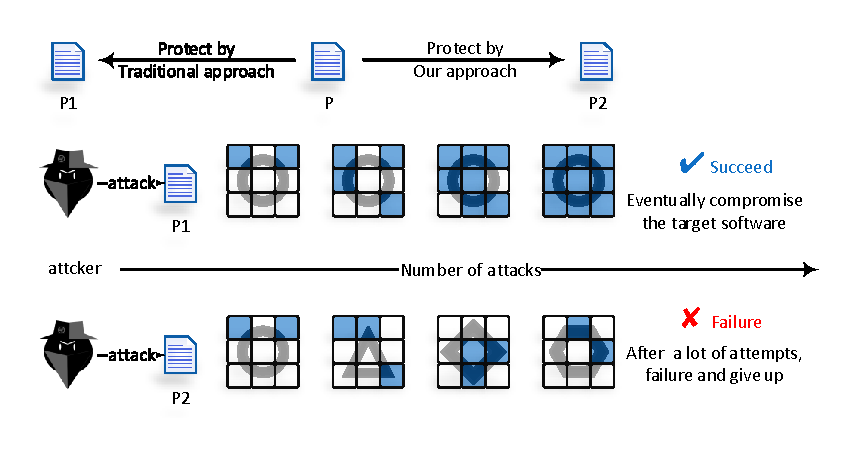
\includegraphics[width=0.7\columnwidth]{figure/figone.pdf}
    \caption{Diversity affects  the attack effectiveness. In this example, a dark small square represents reusable attacking knowledge. Diverse program execution increases the difficulty for performing reverse-engineering based attacks.}\label{fig:Fig.1}
    %\vspace{-5mm}
\end{figure}

\subsection{Our Aim}
As a motivation example, consider Figure~\ref{fig:Fig.1} that illustrates how an attacker
can reuse knowledge extracted from the previous runs of the same application or
other applications that are protected using the same VM scheme to perform an reverse-engineering attack.
This kind of attacks is referred as \emph{cumulative attacks} in this paper.
In the first scenario, the software always follows the same execution path
across multiple runs. Under this setting, the attacker may be able to use a few runs to
obtain sufficient knowledge about the program behavior.
In the second scenario, the program execution path changes across different runs.
As such, it will take longer and many more runs to gather enough information to perform the attack.
As can be seen from this simple illustration, diversity is key for us to protect software against dynamic cumulative attacks.
This is the aim of this work, to improve the diversity of program executions for code obfuscation. 
It is to note that like any other code protection techniques, our approach could be exploited by malware.
How to prevent this is out of the scope of this work. 




\section{The Attack Model}\label{sec:attack}
\subsection{Attacking methods}
The classical approach to reverse engineer a VM-protected program typically
follows three steps~\cite{10falliere2009inside,17rolles2009unpacking}, described as follows.
The first step is to understand how each components of a VM interpreter works.
To do so, the attacker needs to locate
these components and analyze how the dispatcher schedules bytecode instructions for interpretation.
The second step is to understand how each bytecode is mapped to machine code
and work out the semantics of the bytecode instructions, i.e. how will a bytecode opcode 
be translated into a native machine instruction.
The third step is to use knowledge obtained in the first two steps to recover the
logic of the target code region, through removing the redundant information
and generating a simplified program that is equivalent to the original program.


To perform such an attack, a significant portion of the time will have to spend in analyzing the working
mechanism of the VM.
The problem is that a skilled attacker could  reuse knowledge
gathered from parts of the program to analyze other protected regions of
the same program or other applications protected using the same VM scheme and bytecode instructions.

\subsection{Threat model}
Our attack model assumes that the attacker has the necessary tools and skills to implement the above reverse-engineering based attacks.
We assume the adversary holds an executable binary of the
target software and can run the program in a control
environment~\cite{11collberg2002watermarking}. We also assume the adversary
can access content stored in memory and registers, trace and modify program
instructions and control flows.
All these can be achieved using profiling and analysis tools like ``IDA"~\cite{14Idapro}, ``Ollydbg"~\cite{15Ollydbg} and
``Sysinternals suite"~\cite{16Sysinternalssuite}. The aim of the adversary is
to completely reverse the internal implementation of the target program.
Our goal is to increase the difficulties in terms of time and efforts for an adversary to
reverse the target program implementation protected using VM-based code obfuscation. 
\section{Overview of Our Approach}\label{sec:overview}
To address the problem of cumulative attacks, we want to introduce a certain
degree of diversity and uncertainty into program execution. This is achieved
through using a diversified scheduling structure (Section~\ref {sec:dvs}) and
multiple VMs (Section~\ref {sec:mvm}). Like other VM-based protection schemes,
\DSVMP focuses on protecting critical code regions but not the entire program to minimize the runtime overhead.
Figure~\ref{fig:Fig.overview} depicts the system architecture of \DSVMP.
Code protection of \DSVMP follows several steps described as follows.

\begin{figure}[!t]
  \centering
  % Requires \usepackage{graphicx}
  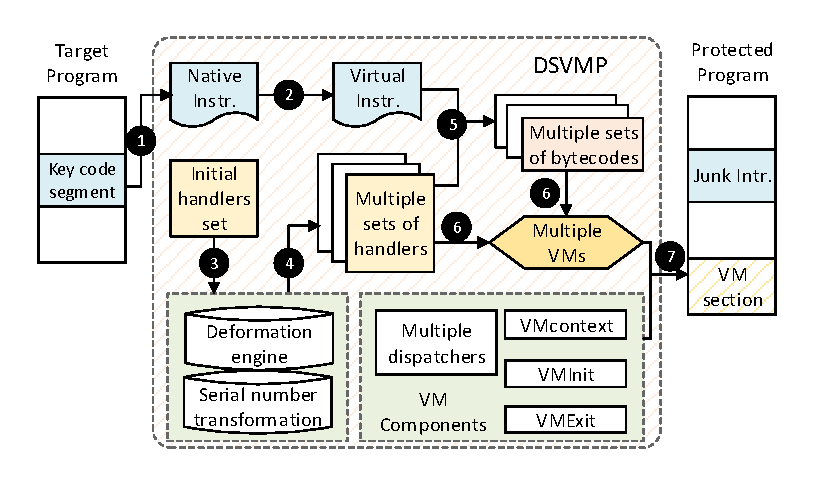
\includegraphics[width=0.7\columnwidth]{figure/figoverview.pdf}
  \caption{Offline code protection process. \DSVMP takes in a program binary. For each protected code region, it translates native instructions into bytecodes. Next, it generates multiple bytecode handlers that are semantically equivalent but implemented in different ways. It then generates the corresponding driver-data and multiple VMs. Finally, the generated VMs and associated components will be inserted into the program binary and fills the original code region with junk instructions.}\label{fig:Fig.overview}
  %\vspace{-5mm}
\end{figure}

\paragraph*{Code translation} \DSVMP takes in a compiled program binary and
does not require having access to the source code. Code segments need to be
protected are given by providing the symbolic name of the functions or a pair
of the start and end address in the binary file. The code segments are
firstly converted into native machine assembly code (e.g. x86 instructions)
using a disassembler (Step \ding{182}), which will then be mapped into a set of virtual instructions (Step \ding{183}).

\paragraph*{Diversifying}
As a departure from prior work on VM-based code obfuscation, \DSVMP employs multiple VM instruction scheduling policies
where each scheduler can have multiple dispatchers and handlers. It provides a set of handlers 
that are semantically equivalent but  are implemented in different ways for a single virtual instruction. 
Thus, the scheduler can dynamically determine at runtime which of the handlers is used to interpret a virtual instruction. 
Multiple handlers are generated by applying obfuscation to a set of seed handlers (Step \ding{184}).
The way the handlers are obfuscated could be different for different code regions.
\DSVMP uses a multi-VM schemes with more than one VM implementation. 
Therefore, each handler will be obfuscated for each VM by using the deformation engine \FIXME{What is the deformation engine and what is VMNum?}, resulting in $n$ (the number of VMs) sets of semantically equivalent handlers with different implementations and control flows (Step \ding{185}). 
Next, the virtual instructions will be encoded into different sets of bytecode for each VM. In our current implementation, the virtual instructions
are encoded into two different sets of bytecode for each VM implementation (Section~\ref {sec:mbd}), i.e. $2*n$ sets of bytecode for $VMNum$ VMs (Step \ding{186}). Subsequently, \DSVMP constructs multiple VMs, where each VM contains one set of handlers (where a virtual instruction
can be interpreted by multiple handlers), and two sets of bytecodes (Step \ding{187}).

\paragraph*{Code generation}
Finally, a new section will be inserted into the program binary, which contains $VMNum$ VMs and their components such as dispatchers, VMContext etc. It also fills the original code region with junk instructions (Step \ding{188}).

This is an overview of our approach. We describe the implementation of \DSVMP in more details in the following sections.



\section{\DSVMP Scheduling Structure}\label{sec:dvs}

The \DSVMP VM scheduler uses multiple dispatchers to determine which bytecode instruction should be interpreted at given time.
A unique design of \DSVMP is that the dispatcher used to schedule bytecode handlers will be dynamically changed at execution time. To further increase the diversity of program behaviour, \DSVMP also uses multiple bytecode instruction sets and bytecode handlers.

\subsection{Multiple Bytecode Handlers}\label{sec:mb}

\begin{figure}[t!]
\scriptsize
\begin{lstlisting}
lods byte/word/dword ptr ds:[esi]
... ...
push eax
rdtsc                    ;------------------------
mov ecx,2
div ecx                  ;structure control unit
cmp edx,0
jz label                 ;------------------------
lods dword ptr ds:[esi]
... ...                  ; to the next handler
add dword ptr ds:[edi+48],eax
jmp dword ptr ds:[edi+48]
label: push ebx          ;------------------------
div bl
movzx eax,AH             ; return to a dispatcher
add eax,9dH
\end{lstlisting}
%\vspace{-2mm}
\caption{Each bytecode handler has a control unit that randomly determines whether the control after exiting the handler should be given to a dispatcher or an alternative bytecode handler. }
%\vspace{-5mm}
\label{fig:newhandler}
\end{figure}

In classical VM-based code obfuscation, a single dispatcher is responsible for fetching a bytecode instruction and
determining which bytecode handler should be used to interpret the instruction by checking the opcode of the bytecode
instruction.
Because each bytecode instruction
is decoded by a fixed handler set, an adversary can easily work out the mapping from an opcode to its
handler. From the mapping, the adversary can correlate the native machine code to each bytecode to analyze the
program behavior and  the logic structure.

To address this issue, for each bytecode handler, we use obfuscation techniques to automatically generate a number of alternative implementations which all
produce an equivalent output for the same input instruction. Different implementations, however,
are programmed in different ways using e.g. different control flows, data structures or obfuscation methods.

To control the program execution path, we insert a control unit at the end of each bytecode handler. Before exiting a bytecode handler,
the control unit randomly determines whether the control should be given back to a dispatcher or
another handler. Figure~\ref{fig:newhandler} shows an example of the control unit of a \DSVMP bytecode handler.
The control unit (lines 4-8) randomly determines to execute the code at line 9 or line 13.
At line 9 , the ``\texttt{lods}" (a load operand in the x86 assembly) instruction fetch an offset value
to calculate the address of an alternative bytecode handler and jump to execute it.
By contrast, the instruction at line 13 will return to a dispatcher.

\begin{figure}[!t]
  \centering
  % Requires \usepackage{graphicx}
  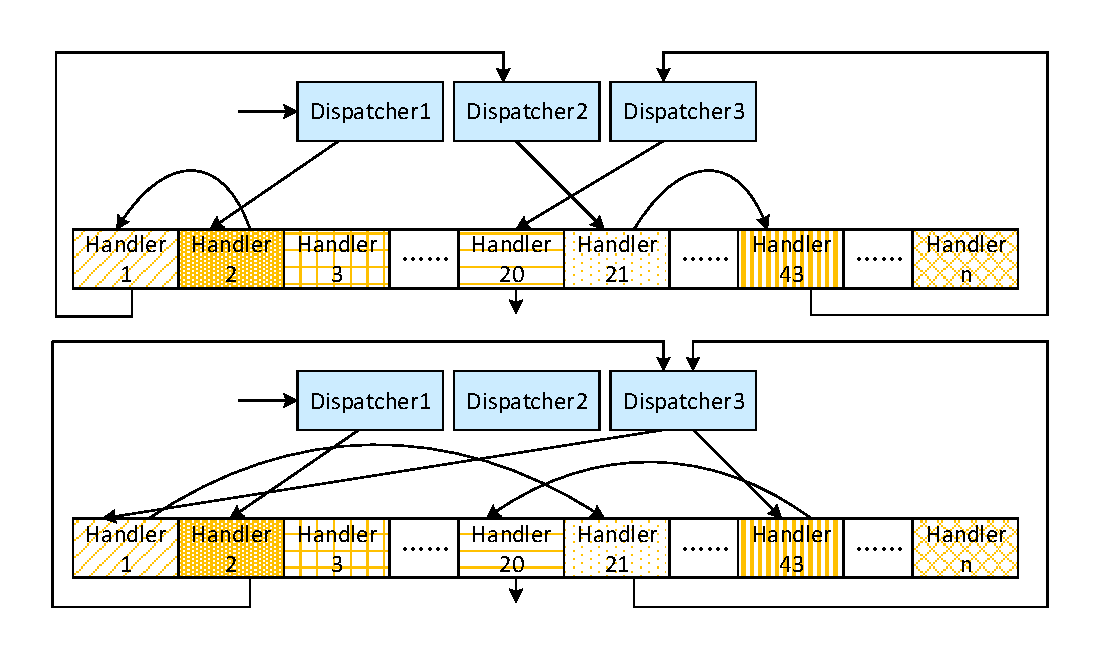
\includegraphics[width=0.65\columnwidth]{figure/figdh.pdf}
  %\vspace{-1mm}
  \caption{Using multiple dispatchers and insert a control unit to handlers increases the diversity of program executions. In this example, the type of handlers and the order of them are called are different across execution runs. }\label{fig:Fig.dh}
  %\vspace{-3mm}
\end{figure}

\subsection{Multiple Bytecode Formats and Dispatchers}\label{sec:mbd}
\paragraph{Bytecode Formats} Using VM-based obfuscation, the protected code regions will be translated into virtual
instructions and stored in a bytcode format. A handler will
be chosen to decode the bytecode instruction to translate it
to native machine code at runtime.  In classical VM-based
code obfuscation approaches, there is one-one mapping from a
bytecode opcode to a handler, i.e. the bytecode opcode
determines which handler to be used.
Having multiple
bytecode instruction sets for different code regions of a target program can provide stronger protection.
By doing so, the same opcode from different code region will have
different semantic meaning as the same opcode from different regions can be mapped into different handlers and hence different
native machine code. For this reason, the virtual instructions
of different  code regions will be stored in different bytecode formats.

As a proof of concept, our current implementation uses two bytecode formats for each VM,
namely \emph{DriverData1} and \emph{DriverData2}. Additional bytecode formats
can be easily added to our system.
Here, \emph{DriverData1} is a
standard bytecode format where each bytecode consists of the
virtual instruction's opcode (a ID indicates which handler should use to
interpret the virtual instruction) and their operand. \emph{DriverData2} has a different
format compared to \emph{DriverData1}. The first data of \emph{DriverData2}
is the handler's ID, The rest of \emph{DriverData2} include the
offset value between two adjacent handlers (for example, handler21 and handler43 in Figure~\ref{fig:Fig.dh}) and their operand.
Recall that a control unit is inserted to the end of each handler to determine
whether the control should be given back to the dispatcher or another handler.  Before exiting the handler,
if the control unit chooses to execute the next handler, it will fetch the corresponding offset value from \emph{DriverData2}.

\paragraph{Dispatchers} \DSVMP also provides multiple dispatchers to further increase the diversity of program execution.
As an example, considering  Figure~\ref{fig:Fig.dh} which
shows two possible program execution paths using three dispatchers within a single VM. As can be seen
from the diagram, a handler can either be invoked by a dispatcher or another handler;
and the type of handlers to be invoked and the order they are called could be different in two different execution runs.
As a result, knowledge about the program control flow extracted from the first run does not apply to the second one.


\section{Multiple VMs}\label{sec:mvm}
In contrast to classical VM-based obfuscation approaches that uses a single VM, \DSVMP uses multiple VMs.
Multiple VMs offer different sets handlers and bytecode instruction sets. Under such settings,
bytecode instructions can be scheduled from different VMs and a virtual instruction can be interpreted by more than one handler.
Therefore, there will be more than one mapping from a bytecode instruction to handlers.
Together with the above multiple scheduling approach, multiple VMs can further increase the diversity and uncertainly of program execution.

\begin{figure}[!t]
  \centering
  % Requires \usepackage{graphicx}
  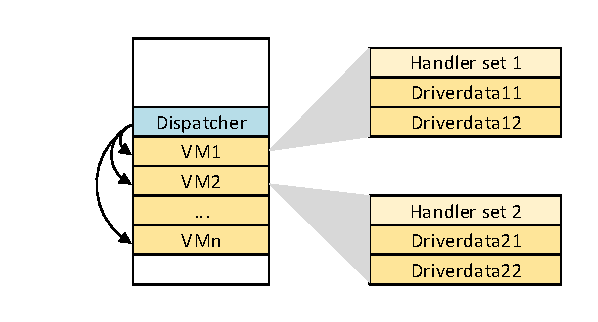
\includegraphics[width=0.6\columnwidth]{figure/figmvm.pdf}\\
  \caption{The structure of multiple VMs. Each VM has one set of unique handlers and two sets of bytecode instructions, \emph{DriverDataSetN1} and \emph{DriverDataSetN2}.}\label{fig:Fig.mvm}
  %\vspace{-2mm}
\end{figure}


\subsection{Switching between VMs}
In \DSVMP, the number of VMs to use is a  parameter that can be configured by the user. This number can vary
depending on the target program to be protected, and the trade-off between the protection strength and runtime overhead.
As described in Section~\ref{sec:mbd}, we generate a set of handlers for each VM so that
we have $n$ different sets of handlers for $n$ VMs. Our current implementation
also stores the virtual instructions of each protected code region using two different bytecode formats. 
The same opcode will have different semantics in different VMs. 

Our system dynamically determines which VM to use to translate a bytecode at runtime. 
This is done through altering the structure of the instruction dispatcher
which decides which VM to use.
To switch to another VM, we first calculate the address offset between the current VM and the next VM to use.
%\FIXME
Our implementation uses the x86 \texttt{ESI} register as a program counter to store the
address of the current bytecode instruction. In order to switch to another VM,
we can simply store the address of the next VM into \texttt{ESI}.
%We then store the value of the x86 register \texttt{ESI} (which is used as a program counter for storing the address of the current bytecode instruction)
%and change the pointer of the new bytecode address according to the offset value.
\FIXME{Is this ESI register implementation dependent? Could your implementation uses other registers? If so, explain this!!!}
Figure~\ref{fig:Fig.mvm} shows the multiple VM structure. \FIXME{The diagram doesn't really say anything. We need to update it
to show the process of VM switching.}
The VM, the set of bytecode handlers and bytecode instructions will be randomly switched
across different code regions in both a single execution and across different program runs.
\FIXME{Since each VM has its handler set, how can you guarantee the same bytecode will give the same 
native code in different VMs? -- This section needs a lot of attentions. }

\subsection{The VM Scheduling Process}\label{sec:mvm-2}
%VM-based protection system uses its own virtual interpreter to interpret the special bytecode program into the native code
%(by scheduling various handlers to implement discrete sub operations) to realize the function of the original target code.
We add the special control unit in the execution process of virtual interpreter, its main works are as follows:
\begin{itemize}
  \item structure control unit determines whether the control should be given to a dispatcher or another handler randomly.
  \item multi-VM switcher determines which VM to use at runtime randomly.
\end{itemize}
\FIXME{I have no idea of what you are talking here. Please rewrite the sentences to make it clear. Considering
why you want to do this, what's the challenge of doing this, how did you solve these challenges?}

In multiple VMs, all of the handler sets are semantic equivlant,
so \DSVMP can ensure that the function of the target program is correct after randomly selecting.
The collaboration of different components achieves the ultimate goal of the strong protection of the original target program,
and the pseudo description of the \DSVMP virtual interpreter shown as follows:

\begin{algorithm}[t!]
\caption{Virtual Interpreter's Work Flow\label{Alg:VMcore-work}}
\begin{algorithmic}[1]
%\REQUIRE
%\ENSURE
\STATE \texttt{VMInit}
\STATE Switcher selects a VM randomly
\STATE Fetch a bytecode from \emph{DriverData1} in current VM
\WHILE {$ bytecode \neq \emptyset$}
\STATE Decoding the bytecode
\STATE JMP handler to interpreter it
\STATE Control unit randomly transfer control
\IF {Choose the \texttt{dispatcher}}
\STATE Select a dispatcher randomly
\STATE Switcher selects a VM randomly
\STATE Fetch the next bytecode from \emph{DriverData1} in current VM
\ELSE [Choose the next \texttt{handler}]
\STATE Fetch the next bytecode from \emph{DriverData2} in current VM
\ENDIF
\ENDWHILE
\STATE \texttt{VMExit}
\end{algorithmic}
\end{algorithm}

Algorithm~\ref{Alg:VMcore-work} gives the work flow of virtual interpreter.
When the target program entering the VM, virtual interpreter will fetch the bytecode from \emph{DriverData}
and dispatch the handler to interpret it.
When all the bytecodes are interpreted, the function of original target code also will be implemented.
In this process, the role of the switcher is randomly switches the VM at runtime,
and the control unit will randomly change the scheduling and execution structure of current VM at runtime.
So our \DSVMP can exploit the dynamic scheduling for VM-based protection at runtime.
Such run time diversity can effectively increase the difficulty of the reverse analysis and resist the cumulative attacks.


\section{Example}\label{sec:case}
We use the x86 code snippet shown in Figure~\ref{fig:examplecode} as an example to illustrate how \DSVMP operates.
``\texttt{STARTSDK}" and ``\texttt{ENDSDK}" are used to mark the begin and end of the code region respectively,
and ``00401036" and ``00401038" are the address the two assembly instructions.

\begin{figure}[t!]
\scriptsize
\begin{lstlisting}
STARTSDK
00401036 mov eax, ebx
00401038 sub eax, 03
ENDSDK
\end{lstlisting}
%\vspace{-2mm}
\caption{Example assembly code snippet for a code region to be protected.}
%\vspace{-4mm}
\label{fig:examplecode}
\end{figure}

\subsection{Process of protection}
Firstly, \DSVMP extracts the critical code from the target program that disassembled into native instruction, here will automatically insert two additional instructions (``\texttt{push 0x40103b}" and ``\texttt{ret}") after two key
instructions in order to jump back to execute the native code
after the protected code region, as showed in figure~\ref{fig:examplecode}.
It then converts the native instructions to virtual instructions according to a translation convention.
The resulted virtual instructions is given in Table~\ref{tab:Tab.1}.
\DSVMP's bytecode instructions are based on a stack machine model.
Here the \texttt{load} instruction is used to push operands into the stack,
and the \texttt{store} instruction is used to pop results out from the stack
and store the result to the virtual context (VMContext).

\begin{table}[!h]
\scriptsize
\begin{center}
\caption{Generated virtual instructions for the example shown in Figure~\ref{fig:examplecode}\label{tab:Tab.1}}
{\tabcolsep6pt\begin{tabular}{@{}cllll@{}}
  \hline
    & \textbf{Instr.1} & \textbf{Instr.2} & \textbf{Instr.3} & \textbf{Instr.4} \\
  \hline
  \textbf{ NI} & \texttt{mov eax, ebx} & \texttt{sub eax, 0x03} & \texttt{push 0x40103b} & \texttt{ret} \\
  \hline
  \textbf{ VI} & \tabincell{l}{\texttt{move 0x08}\\\texttt{load}\\\texttt{move 0x04}\\\texttt{store}} & \tabincell{l}{\texttt{move 0x04}\\ \texttt{load}\\ \texttt{load 0x03}\\ \texttt{sub}\\ \texttt{store}\\ \texttt{move 0x04}\\ \texttt{store}} & \texttt{load 0x40103b} & \texttt{ret} \\
  \hline
\end{tabular}}{}
\end{center}
\vspace{-2mm}
Notes: In the table, ``NI" indicates the native x86 instructions, and ``VI" donates the virtual instructions.
Here, our system inserts ``Instr.3" and ``Instr.4" in order to jump back to execute the native code after returning from the protected code region.
\end{table}

After translating the native code to virtual instructions, we use the deformation engine to transform the initial bytecode handlers set. For this example, our system with 2 VMs configurations, so we generate two sets of bytecode handlers which are semantically equivalent but are implemented in different ways.
Then we randomly shuffle the serial numbers of these handlers, resulting in two new sets of handlers: \texttt{HAS1} and \texttt{HAS2}.  Each set of bytecode handlers is associated with two bytecode instruction sets: \emph{DriverDataSet11} and \emph{DriverDataSet12} for \texttt{HSA1} and \emph{DriverDataSet21} and \emph{DriverDataSet22} for \texttt{HSA2}. The resulted program is illustrated in Figure~\ref{fig:Fig.ex}. We store the virtual instructions in the bytecode format,
and will fill the critical code segment to be protected with junk instructions.

Finally, \DSVMP create a new code section attached to the end of the target program.
The new code section contains the implementation of the handlers, different sets of bytecode instructions,
dispatchers and other VM components such \texttt{VMContext} and routines such as
\texttt{VMInit} (used to initialize the VM) and \texttt{VMExit} (use for cleanup before exiting the VM).



\subsection{Runtime execution}
Runtime execution of the protected code region is illustrated in Figure \ref{fig:Fig.ex}, which follows a number of steps:
\begin{itemize}
\item \textbf{Step1:} The entry of the protected code segment contains an ``\texttt{jmp VMInit}" instruction. This transfers the control to the VM initialization routine, \texttt{VMInit}, which saves the native host context and initializes the virtual context.
\item \textbf{Step2:} Next, a dispatcher starts working. It randomly selects a VM, we assume that \texttt{VM2} is chosen at beginning, and then it fetches a bytecode from the \emph{DriverDataSet21}. After decoding, the dispatcher gets a bytecode ``\texttt{6a}". It then jumps to execute ``\texttt{0x6aHandler}", and the next bytecode ``\texttt{07}" is its operand.
\item \textbf{Step3:} A control unit execute (see Section~\ref{sec:mb}) before exiting the ``\texttt{0x6aHandler}". The control unit randomly selects to execute another handler, ``\texttt{0x85Handler}", or return the controller to the dispatcher. If it chooses to return to the dispatcher, the program execution moves to Step 5.
\item \textbf{Step4:} Assume that the control unit decides to direct execute the next handler, ``\texttt{0x85Handler}". It will then fetch a bytecode from \emph{DriverDataSet22}, decoding it and getting the offset address of ``\texttt{0x85Handler}" . Using the offset, the control unit will jump to execute ``\texttt{0x85Handler}". After executing the handler, the program execution moves to Step 3.
\item \textbf{Step5:} If the control unit chooses to return the controller to a dispatcher, it will randomly select a dispatcher to continue the execution. Then, the program moves to Step 6.
\item \textbf{Step6:} The selected dispatcher randomly selects one VM to use. The dispatcher fetches a bytecode from this VM, decoding the bytecode to get the handler serial number.
    It then jumps to execute the handler. After executing the handler, the program execution moves to Step 3.
\item \textbf{Step7:} Step 3 and Step 4 are iterated until all the bytecodes get executed. The finally step is to invoke the \texttt{VMExit} to restore the native context and to continue executing the rest of target program.
\end{itemize}

\begin{figure}[!t]
  \centering
  % Requires \usepackage{graphicx}
  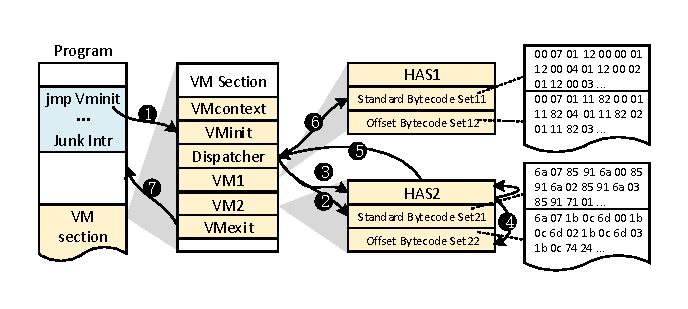
\includegraphics[width=0.7\columnwidth]{figure/figex.pdf}\\
  \caption{The execution process of the protected program. Here each VM has two sets of bytecode instructions and one set of handlers.}\label{fig:Fig.ex}
  %\vspace{-5mm}
\end{figure}

\section{Security Strength Analysis}\label{sec:s-eva}
This section analyzes the security strength provided by \DSVMP. We first analyze the number of possible execution paths. Then we discuss the diversity of code structures.


\subsection{Program execution paths}
Recall that our design goal is to increase the diversity of program execution,
so that in different runts the protected region will not follow a single execution path across runs.
In this analysis, we assume there are 10 different dispatchers. This number matches the current implementation of \DSVMP.
We use the example presented in Section~\ref{sec:case} as a case study.
In this example, \emph{DriverDataSet11} and \emph{DriverDataSet21} each has 103 bytes of data.
They contain a total of 78 handler serial numbers. In this analysis, we exclude the last handler because of it is used to exit the VM.
This leave us 77 handlers where each handler can lead to 11 different execution paths.
This is because at the end of executing each handler, a control unit will determine whether the control
should be given to another handler or one of the 10 dispatchers (see Section~\ref{sec:mb}) -- 11 possibilities in total.

In combination, these options give $11^{77}$ possible execution paths for each protected code region.
Therefore, the probability, $p$, for a protected code region to follow the same execution path across
different runs is $p= \frac{1}{{{{11}^{77}}}}$,
%\[p= \frac{1}{{{{11}^{77}}}}\]
a very small number.
Bear in mind that so far we have assumed that the protection scheme uses just one VM.
The multi-VM strategy employed by \DSVMP further increases the number of possible execution paths.
In fact, the more dispatchers and VMs are, the greater number of possible execution paths will be.
The current \DSVMP implementation provides five different VMs. Together with the multiple dispatchers
and bytecode instruction straggles, for the setting used in this section, \DSVMP gives a single code region
$11^{385}$ possible execution paths. Given the massive number of choices, it will be rare for
a protected code region to take the same execution path across different runs.




\subsection{Code structures}
To prevent an adversary from resuing knowledge obtained from other software to perform attacks,
we would like applications protected by \DSVMP exhibit distinct code structures. In other words,
we would like programs after code obfuscation to be as much dissimilar as possible in terms of code structures.


Blietz \emph{et al.}~\cite{18blietz2006software} proposed a method to measure the similarity of program structures,
using control flow information such as the number of branches and back blocks, the nesting level of the code etc.
We draw lessons from this method to analyze code structures for programs protected using \DSVMP.
We use a number of metrics to describe program code structures. These metrics are:

\begin{itemize}
\item \texttt{NodeNum}: the number of basic blocks of the protected region.
\item \texttt{BranchNum}: the number of basic blocks where the last instruction is a conditional jump instruction.
\item $DR(Vi)$: the number of in and out instructions for the basic block, \emph{Vi}. This metric is defined as $DR(Vi) = {D_{in}}(Vi) + {D_{out}}(Vi)$ where ${D_{out}}\left( {Vi} \right)$ refers to the out-degree and ${D_{in}}\left( {Vi} \right)$ refers to the in-degree and they mean the number of arcs that start or end at $Vi$.
\item $DF(Vi)$: the data flow relationship of basic block, \emph{Vi}. This is used to measure the frequency of \emph{Vi}'s information exchange. It is defined as $DF\left( {Vi} \right){\rm{ }} = {\rm{ }}Flo{w_{in}}(Vi) + Flo{w_{out}}(Vi)$, where $Flo{w_{in}}$ is the number of reading instruction in \emph{Vi} and $Flo{w_{out}}$ is the number of writing instruction in \emph{Vi}.
\end{itemize}


\begin{table*}[!h]
\scriptsize
\begin{center}
\caption{The relevant information about the program\label{tab:Tab.2}}
{\tabcolsep8pt\begin{tabular}{@{}clccccc@{}}\hline
  \multicolumn{2}{c}{\textbf{Basic info of program}} & \multicolumn{5}{c}{\textbf{Info of protected-software}} \\

  \textbf{program} & \textbf{key code segment} & \textbf{program} & \textbf{Node Num} & \textbf{Branch Num} &
  $\sum\limits_{i = 0}^{i < n}{DR(i)}$ & $\sum\limits_{i = 0}^{i < n}{DF(i)}$\\
  \hline
  A & \tabincell{l}{\texttt{mov eax,ebx}\\ \texttt{sub eax,03}} & A' & 23 & 5 & 46 & 18\\

  B & \tabincell{l}{\texttt{pop eax}\\ \texttt{add eax,ebx}} & B' & 48 & 9 & 96 & 36\\
  \hline
\end{tabular}}{
\scriptsize\\Notes: In the table, the number of \texttt{n} which in $\sum\limits_{i = 0}^{i < n}{DR(i)}$
and $\sum\limits_{i = 0}^{i < n}{DF(i)}$ are equal to the \texttt{NodeNum}.}
\end{center}
\end{table*}

Table~\ref{tab:Tab.2} gives two examples of code regions to be protected. These are two simple code snippets and without code obfuscation, these two examples have very similar structures because all of then with just one basic block and no branches. Transforming the code regions using \DSVMP, we obtain different metric values for both code regions,
which indicate the transformed code segments have distinct structures.
We use the following formula to quantify the code structure information, X after code obfuscation.
\[\begin{array}{l}
 SInfo{r_{X}} = NodeNu{m_{X}} + BranchNu{m_{X}} + \sum\limits_{i = 0}^{i < n} {(DR(i) + DF(i))}
 \end{array}\]

Applying this formula for the transformed code segments, A' and  B', listed in Table~\ref{tab:Tab.2},  we get :
\[\begin{array}{l}
 SInfo{r_{A'}} = NodeNu{m_{A'}} + BranchNu{m_{A'}} + \sum\limits_{i = 0}^{i < n} {(DR(i) + DF(i))} \\
                                        = 23 + 5 + (46 + 18)\\
                                        = 92 \\
 SInfo{r_{B'}} = NodeNu{m_{B'}} + BranchNu{m_{B'}} + \sum\limits_{i = 0}^{i < m} {(DR(i) + DF(i))}  \\
                                        = 48 + 9 + (96 + 36)\\
                                        =  189
\end{array}\]

where $n=NodeNu{m_{A'}}$ and $m=NodeNu{m_{B'}}$.
From $SInfo{r_{A'}}$ and $SInfo{r_{B'}}$,
we can calculate the similarity $SDiff$, for two code structure, A' and B' as:
\begin{align*}
SDiff = \frac{{|SInfo{r_{A'}} - SInfo{r_{B'}}|}}{{SInfo{r_{A'}} + SInfo{r_{B'}}}}\;{\kern 1pt}  = \frac{{97}}{{281}} = 34.5\% \end{align*}

Thus it can be seen the code structure similarity between two A' and B' is  34.5\%.
This example shows that \DSVMP can significantly increase the dissimilarity of code structures even for simple code segments.
We also observe that the similarity between transformed code regions drops significantly
as the complexity of original code segments increases.


\section{Performance Evaluation}\label{sec:p-eva}
In this section, we evaluated \DSVMP using four widely use application
and compared it against two commercial VM-based protection systems,
then present the evaluation results of \DSVMP based on the experimental data in detail.

\begin{table*}[!h]
\scriptsize
\begin{center}
\caption{Information of the bechmarks\label{tab:Tab.3}}
{\tabcolsep8pt\begin{tabular}{@{}rlrclrrl@{}}\hline
   & \textbf{program} & \textbf{Size(KB)} & \textbf{Instr. Total} & \textbf{Function to protect} & \textbf{Instr. Protect} & \textbf{Instr. Executed} & \\
  \hline
   & md5 & 11 & 1357 & \texttt{Transform()} & 563 & 229141 & \\
   & aescrypt & 142 & 9788 &\texttt{encrypt-stream()} & 1045 & 478297 & \\
   & bcrypt & 68 & 3081 & \texttt{Blowfish-Encryp()} & 54 & 1050003 & \\
   & gzip & 56 & 9837 & \texttt{deflate()} & 154 & 680037 & \\
  \hline
\end{tabular}}{}
\end{center}
Notes: The 3rd column shown the total number of target program instructions. The 4rd column of the table gives the function to be projected and the 5th column shows the number of instructions of the function. The number of instructions got executed with the critical functions while processing the test file, and shown in the last column of the table.
\end{table*}

\subsection{Evaluation Platform and Benchmarks}
We evaluated \DSVMP on a PC with an 3.0 GHz Intel Core$^{TM}$ 3 Duo processor and 4GB of RAM.
The PC runs the Windows 7 operating system. We evaluated our approach using four widely use applications: ``\texttt{md5}"~\cite{19md5}, ``\texttt{aescrypt}"~\cite{20Aescrypt}, ``\texttt{bcrypt}"~\cite{21bcrypt} and ``\texttt{gzip}"~\cite{22gzip}.
We used these applications to process a test text file. The size of the file is 26 KB.
Table~\ref{tab:Tab.3} gives some information of the protected code regions for each benchmark.
The total number of target program instructions are shown in the 3rd column of the table.
The 4rd column of the table gives the function to be projected
and the 5th column shows the number of instructions of the function.
Finally, we use the Intel Pin tools~\cite{pin} to calculate the number of instructions got executed with the critical functions
while processing the test file, and shown in the last column of the table.


\subsection{Code Size and Runtime Overhead}\label{sec:benchmarktest}
\paragraph*{Code size} For each target benchmark, we applied \DSVMP to the target function and repeated the process for 8 times.
For each protection run, we used a different number of VM configuration.

\begin{figure}[t]
\centering
\begin{minipage}[t]{0.49\linewidth}
\centering
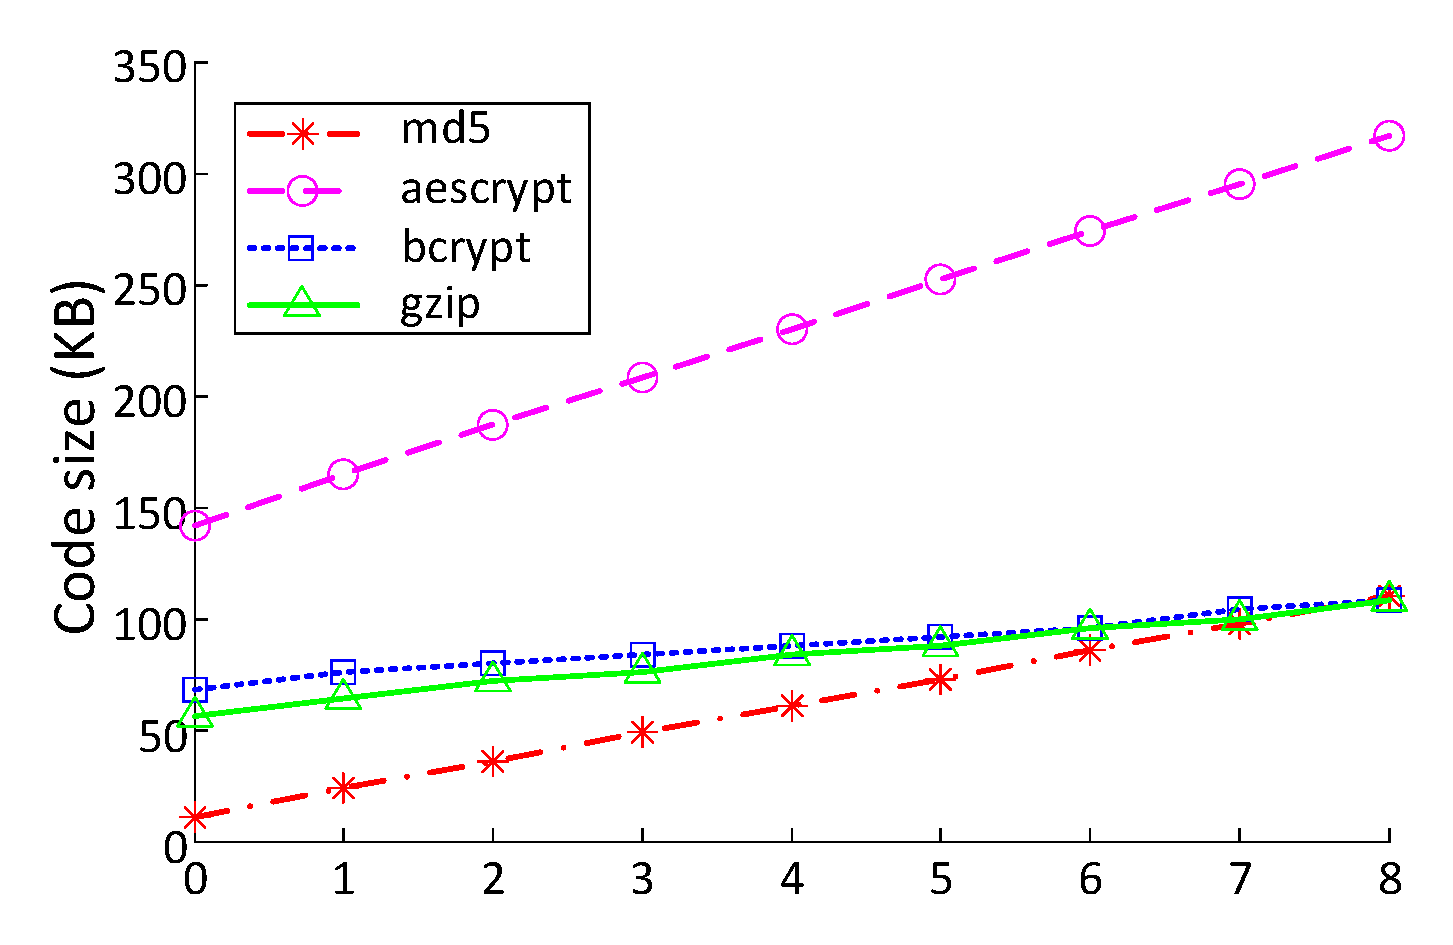
\includegraphics[width=.9\textwidth]{figure/codesize.pdf}
\caption{The impact of code sizes for \DSVMP configurations with a different number of VMs. The number of horizontal axis is the configuration of the VMs, ``0" is the original program.}\label{fig:Fig.size}
\end{minipage}
\hspace{0.005\textwidth}
\begin{minipage}[t]{0.49\linewidth}
\centering
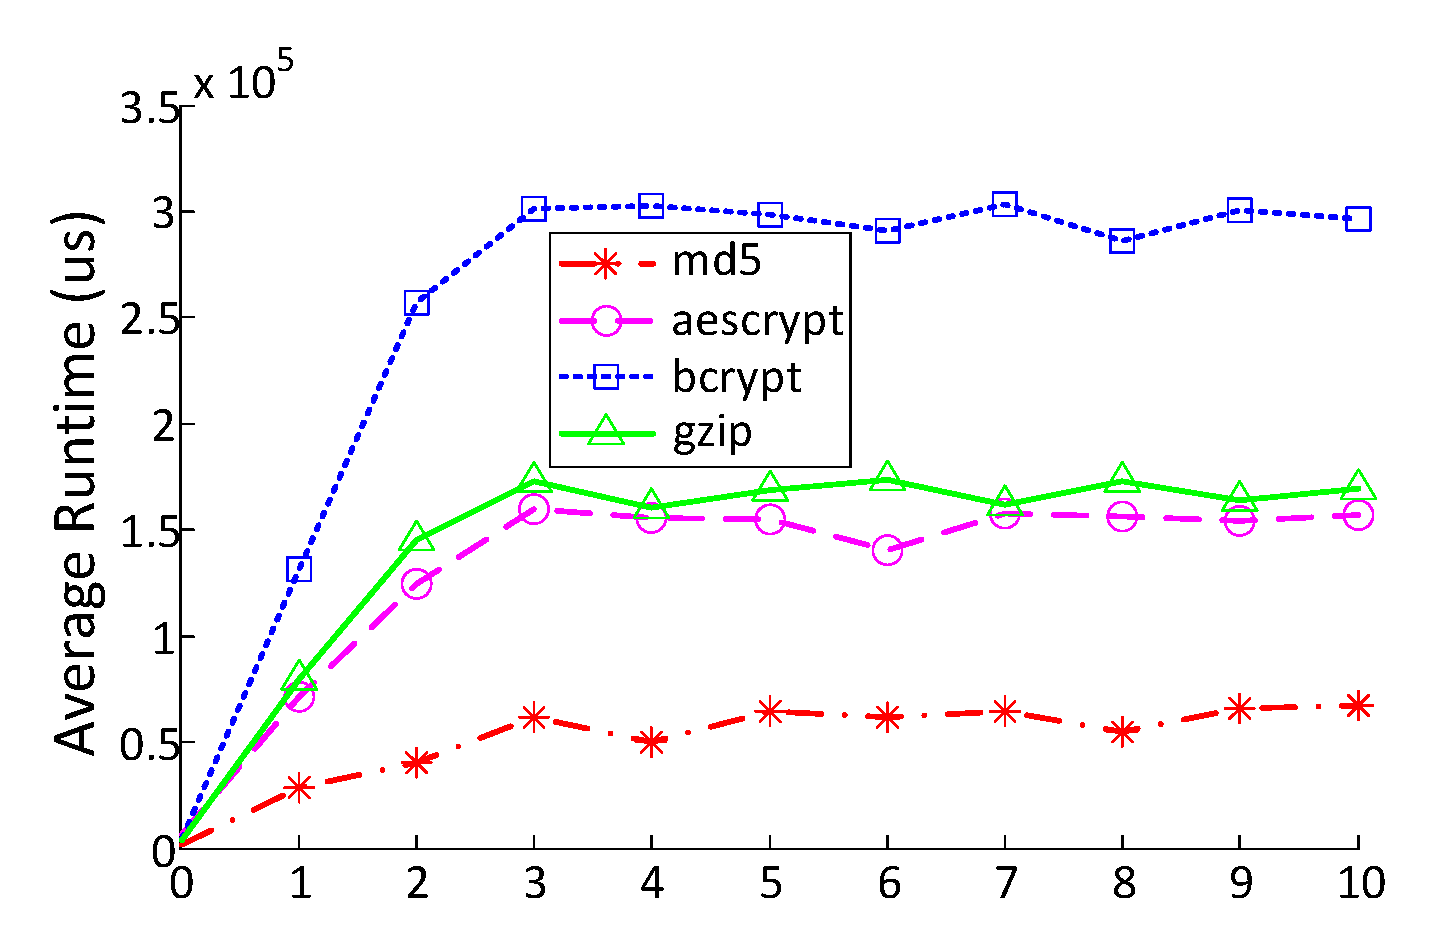
\includegraphics[width=.9\textwidth]{figure/runtime.pdf}
\caption{The average runtime of target benchmark when protected with different VMs. The number of horizontal axis is the configuration of the VMs, ``0" is the original program.}\label{fig:Fig.time}
\end{minipage}
\end{figure}


Figure~\ref{fig:Fig.size} shows how the \DSVMP multi-VM scheme affects the code size,
and the number ``0" represents the original target program.
As described before, each VM has two bytecode instruction sets and one set of handlers,
the code size of the protected program grows as the number of VM increases.
Obviously, the increase in code size is regular, because the block of PE executables
are usually follow a certain alignment value (such as, 4096 or 512)~\cite{pe}.

Moreover, we can find that there is a strong correlation between the code size of and the number of protected instructions.
This explains why ``\texttt{aescrypt}" has the fastest increase of code size as it has
the largest number of protected instructions (see Table~\ref{tab:Tab.3}).
For the same reason, the code size of ``\texttt{bcrypt}" grows slower than other programs,
as this benchmark has the least number of protected instructions.


\paragraph*{Runtime overhead} To evaluate the runtime overhead of \DSVMP, we used benchmark to process the test file.
For each protected benchmark we repeated the process for 10 times and report the average runtime per benchmark.

The results are depicted in Figure~\ref{fig:Fig.time},
which shows that the majority of average runtime will tend to a stable range with the increase of the number of VMs.
This phenomenon is inevitable, the increase in the number of VMs leads to a
greater likelihood and diversity of handler's choice, when interpret the virtual instructions.
It does not add a lot of extra operations to the core function implementation.
The main reason for the impact of runtime overhead is the switching of multiple VMs
and the execution difference of obfuscated handler.
As the number of VMs increases, the frequency of VM switching tends to stabilize,
so the impact of different VM on the time is different but tends to a stable range.

Besides, we found that the greater the execution number of the protected instruction at runtime
will have a greater impact on runtime overhead.
This is why ``\texttt{bcrypt}" has a much higher runtime overhead than other benchmarks.

There is also a special phenomenon that compared to other protection strategies,
2-VM increase in running time overhead is not obvious.
This is due to the fact that the random policy we are using does not frequently switch VM in a 2-VM configuration.
Therefore, its impact on time overhead will not be obvious.
We have done the relevant test experiments to validate it, see Section~\ref{sec:s-d} for details.


\paragraph*{Discussion}
Comprehensively assess the experimental results of several target benchmarks in table~\ref{tab:Tab.3}.
We find the temporal and spatial overhead of the target program is mainly affected by
the size of the key code and the number of instructions at execution time.
So we have reason to believe, if we only focus on protecting a few critical code regions,
\DSVMP will not cause too much impact on the temporal and spatial overhead of the target program.


\subsection{Structural diversity}\label{sec:s-d}

\paragraph*{Multi-VM switching test}
In order to verify the impact of multi-VM switching on program execution, we did a runtime tracking experiment.
We only protected one instruction ``\texttt{mov eax, 1234567}" for ``\texttt{test.exe}"\footnote{A small test procedures, size of 3 KB, and its function is to pop up a confirmation box.}.
So as to reduce the complexity of the protected program as much as possible to facilitate the tracking procedures.
We use three kinds of strategy (2-VM, 3-VM and 4-VM) to protect the target program,
and then track the program execution 5 times and collect the relevant information.


\begin{figure}[t]
\centering
\begin{minipage}[t]{0.49\linewidth}
\centering
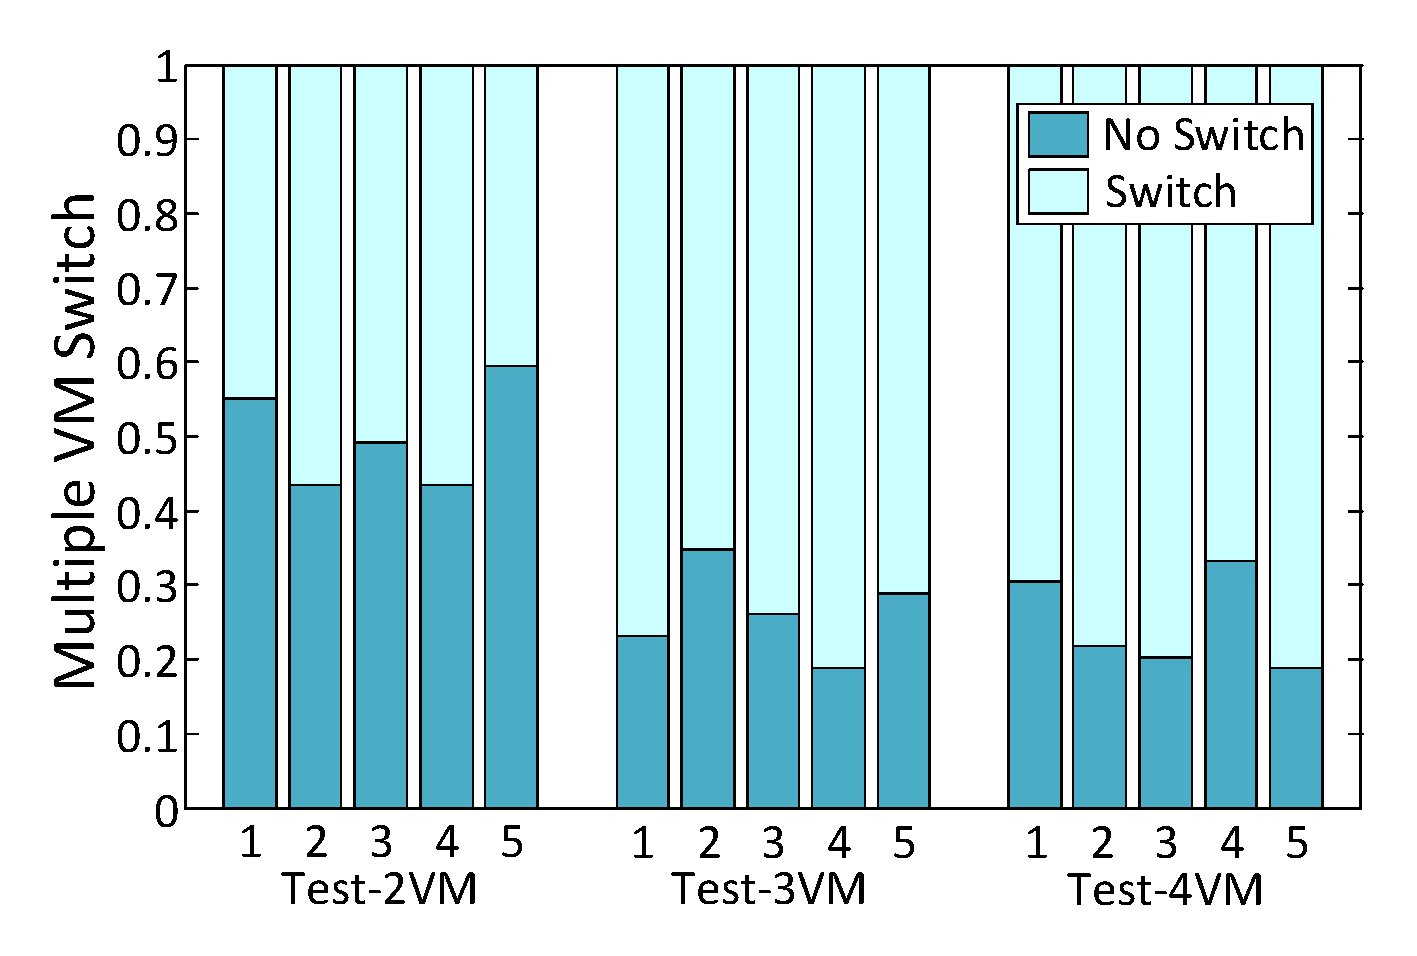
\includegraphics[width=.9\textwidth]{figure/testinfor.pdf}
\caption{The probability distribution of multiple VMs switching for multiple runs. ``Switch" is the number of times the VM switch, and ``No Switch" is the opposite.}\label{fig:Fig.testinfor}
\end{minipage}
\hspace{0.005\textwidth}
\begin{minipage}[t]{0.49\linewidth}
\centering
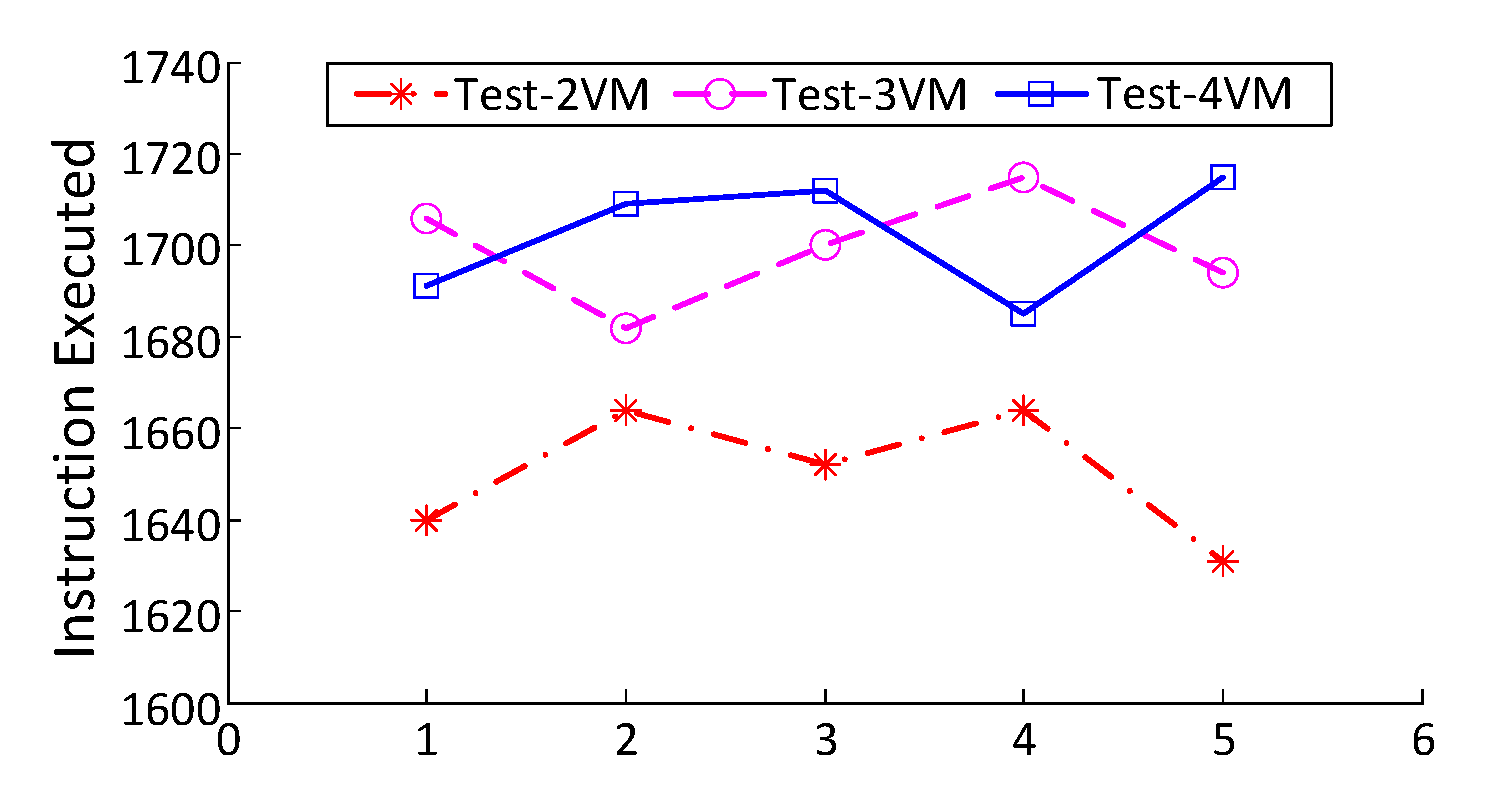
\includegraphics[width=.9\textwidth]{figure/testinstr.pdf}
\caption{The number of instruction dynamic executions changes with different VM configurations. Here it is mainly affected by the Multiple VM switch.} \label{fig:Fig.testinstr}
\end{minipage}
\end{figure}


Figure~\ref{fig:Fig.testinfor} shows the VM switching frequency information of ``\texttt{test.exe}" at five actual execution. A total of 69 times handler scheduling are required to implement the test key instruction functions.
We found that the frequency of VM switching is not high when the number of VMs is 2,
unlike the 3-VM and 4-VM of the switching frequency has exceeded 75\%.
In particular, we removed handler obfuscation and used only one dispatcher in the protection process.
This can minimize the impact of irrelevant factors, and then only the multi-VM switcher can affect the number of instruction executed.
Through the experiment we found that the impact of 2-VM on the number of instructions got executed is less than 3-VM and 4-VM,
as the figure~\ref{fig:Fig.testinstr} shows.
In general, the number of instruction execution can be reflected to some extent the size of the execution time.
So this can also explain why the 2-VM has a smaller effect on runtime overhead in figure~\ref{fig:Fig.time}.

\begin{figure}[t]
\centering
\subfigure[]{
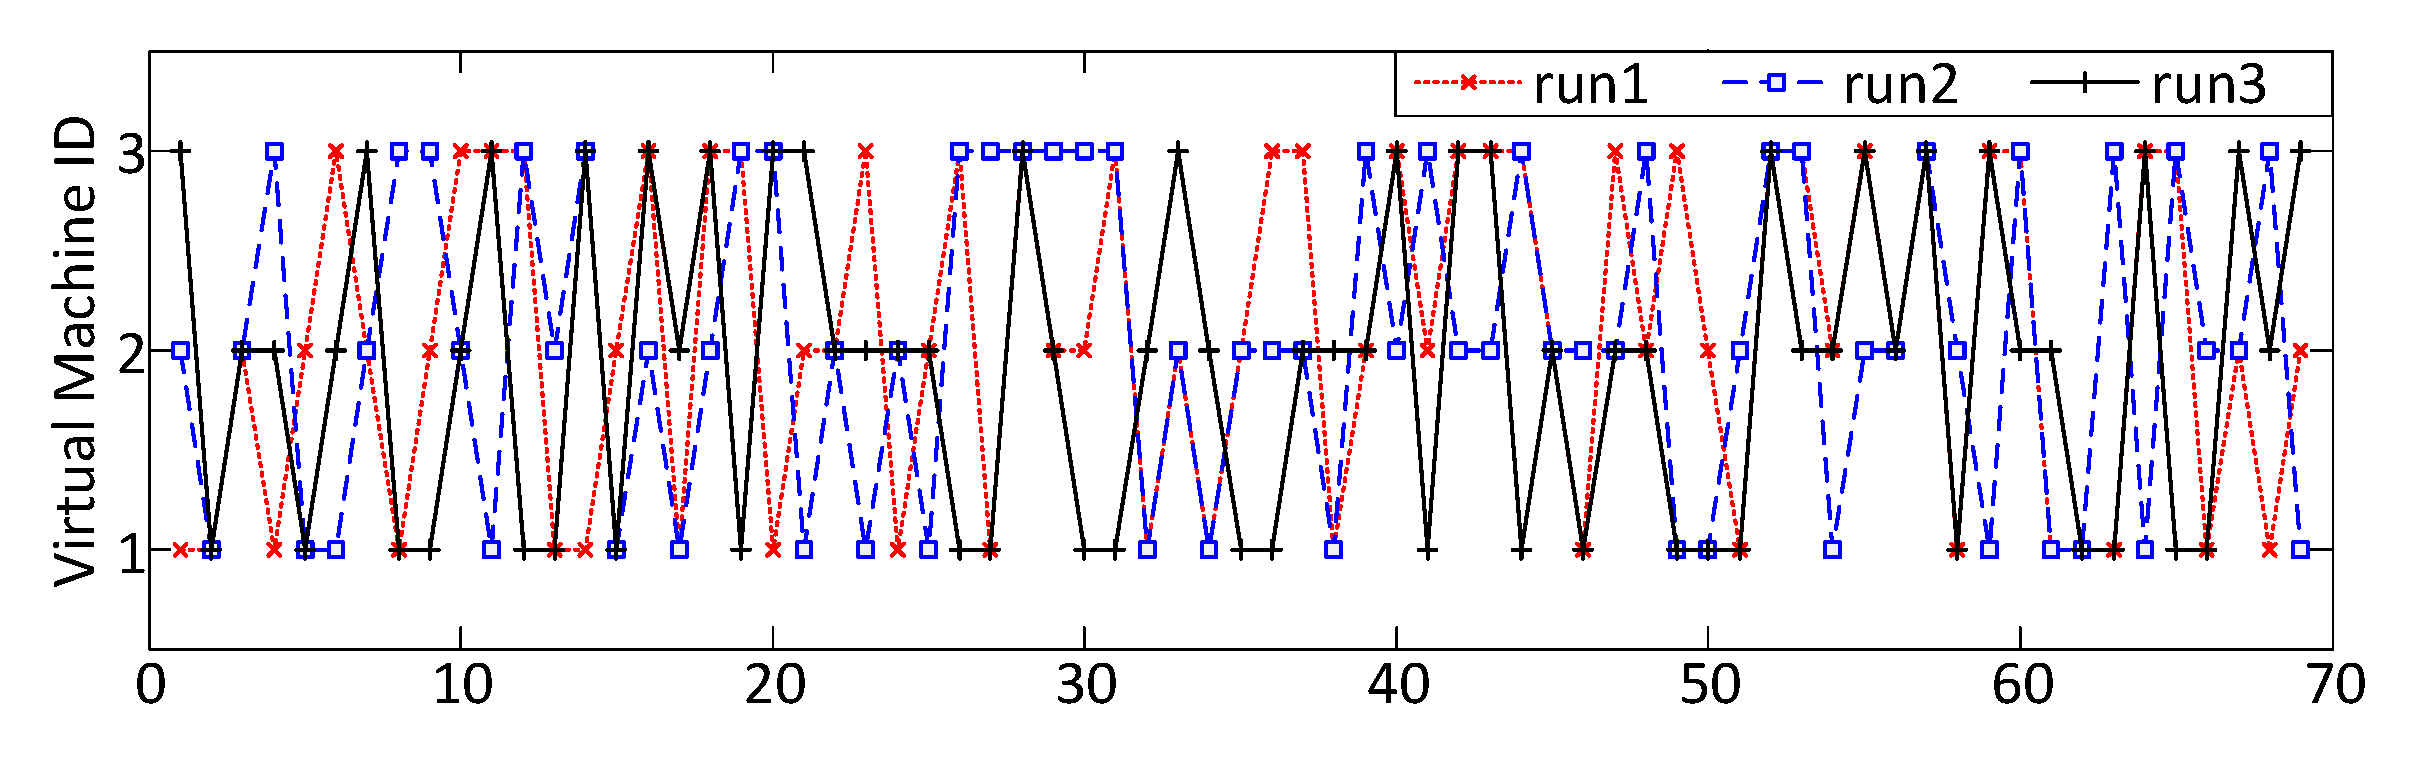
\includegraphics[width=0.485\textwidth]{figure/exec3vm.pdf}}
\subfigure[]{
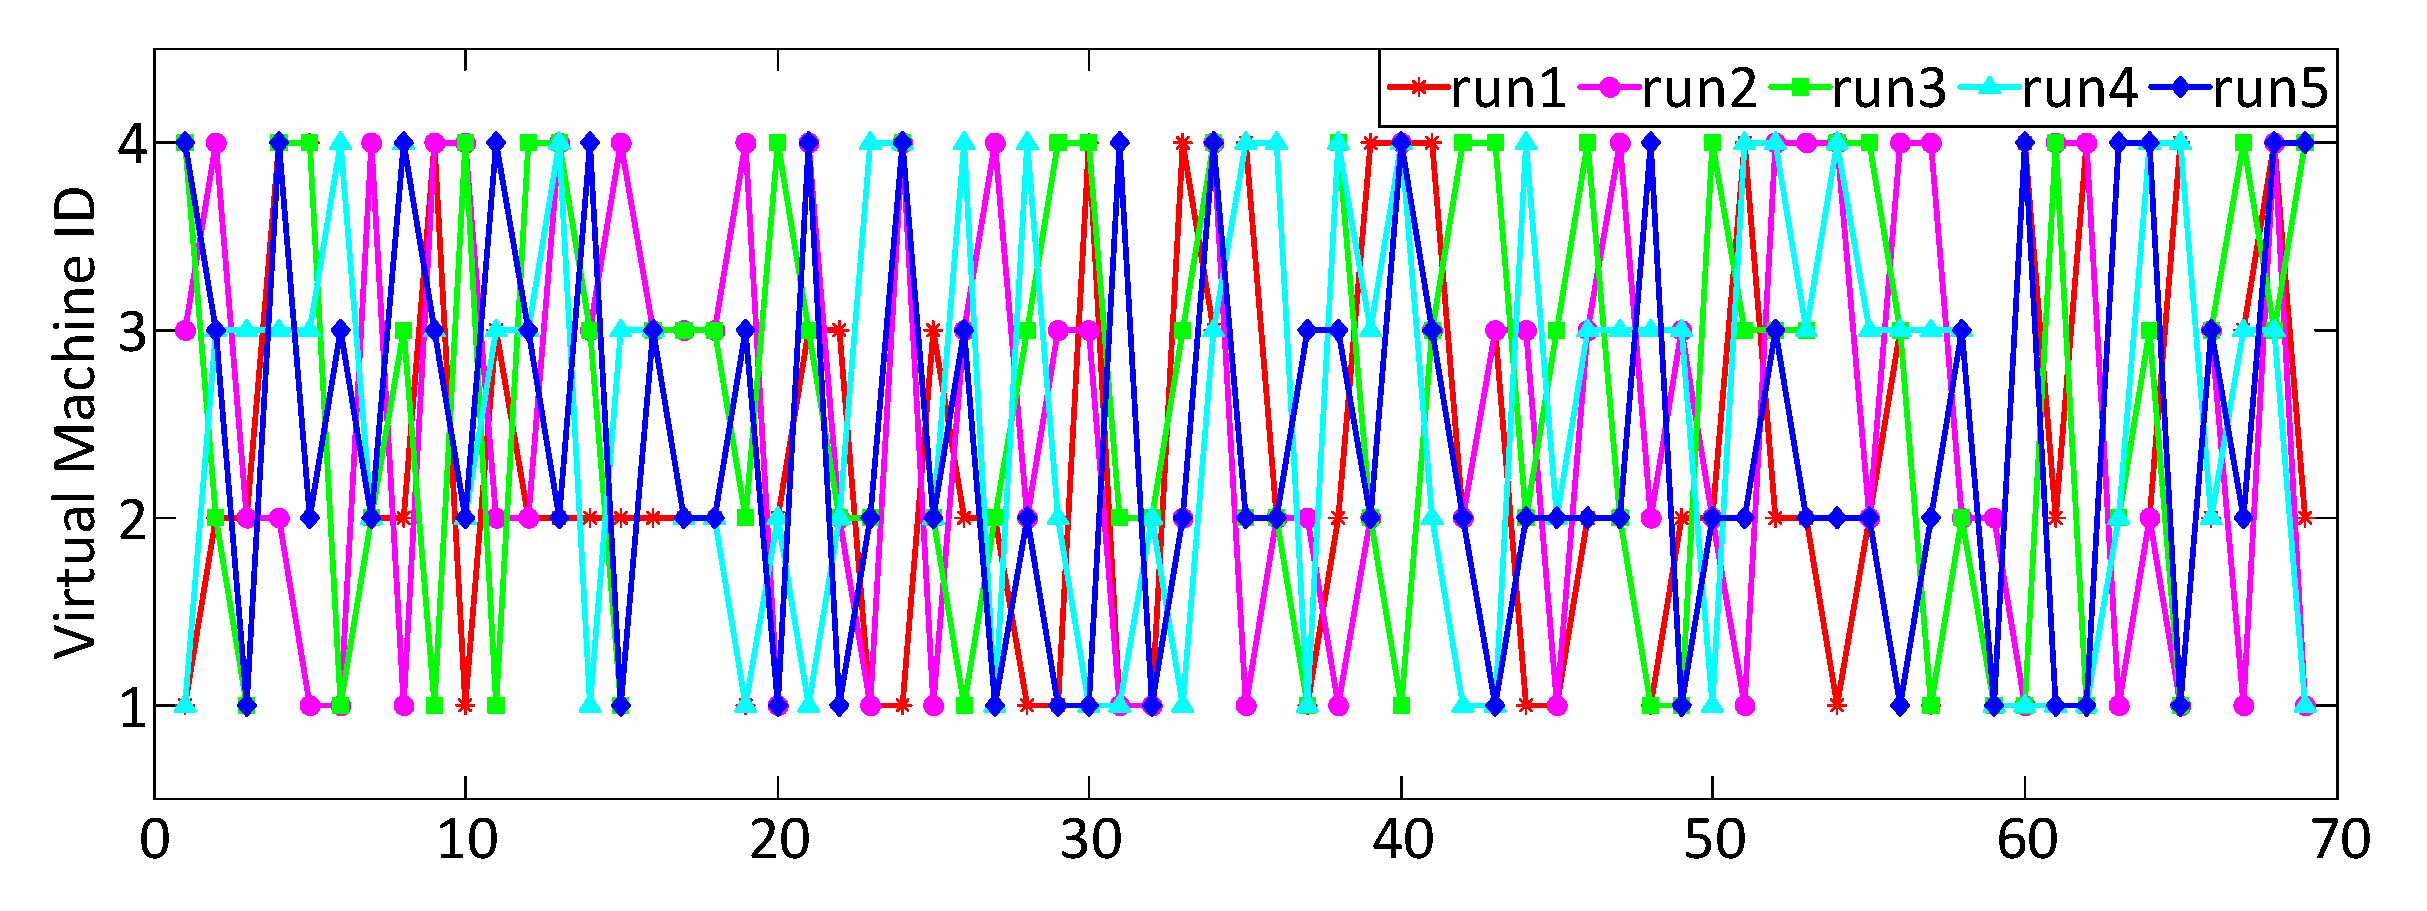
\includegraphics[width=0.485\textwidth]{figure/exec4vm.pdf}}
\caption{Dynamic VM switching during the protected program execution. The handler's scheduling order is plotted on the abscissa, starting at the origin and moving to the right. There are a total of 69 schedules. The value on the ordinate corresponds to VM's ID which is selected for each schedule. Lines of different colors show the true change of the VM in 5 executions. (a) is ``Test-3VM", and (b) is``Test-4VM". }\label{fig:Fig.execvm}
\end{figure}

\paragraph*{Perform path runtime diversity}
In the course of the above experiment, we also collected the ID of the VM where the handler was executed each time.
Figure~\ref{fig:Fig.execvm} shows the switching of the VM for five runs.
The data in (a) and (b) are from the test program with 3-VM and 4-VM configurations, respectively.

As can be clearly seen in the figure, VMs are randomly selected for different runs,
and the path of execution 5 times is completely different. As alluded to earlier (section~\ref{sec:mvm}),
the set of handlers in each VM is confused with different obfuscation methods and is combined in an out-of-order manner.
Therefore, the structure of the called Handler is different for the same phase of the different runs.
Take 4-VM configuration test program as an example, a total of 69 Handlerd scheduling,
regardless of the middle of the dispatcher changes in the process,
only the Handler scheduling execution there is $4^{69}$ different execution path.
This value is very large, and it will be great resistance to the adversary who use cumulative attacks.

\paragraph*{Discussion}
According to the experimental results, we can see, the execution path of a protected program is variable at runtime.
Combined with various handler sets, the target program protected by \DSVMP has temporal diversity~\cite{4collberg}.
Therefore, our approach can effectively resist the cumulative attacks.

%\begin{figure}[!t]
%\centering
%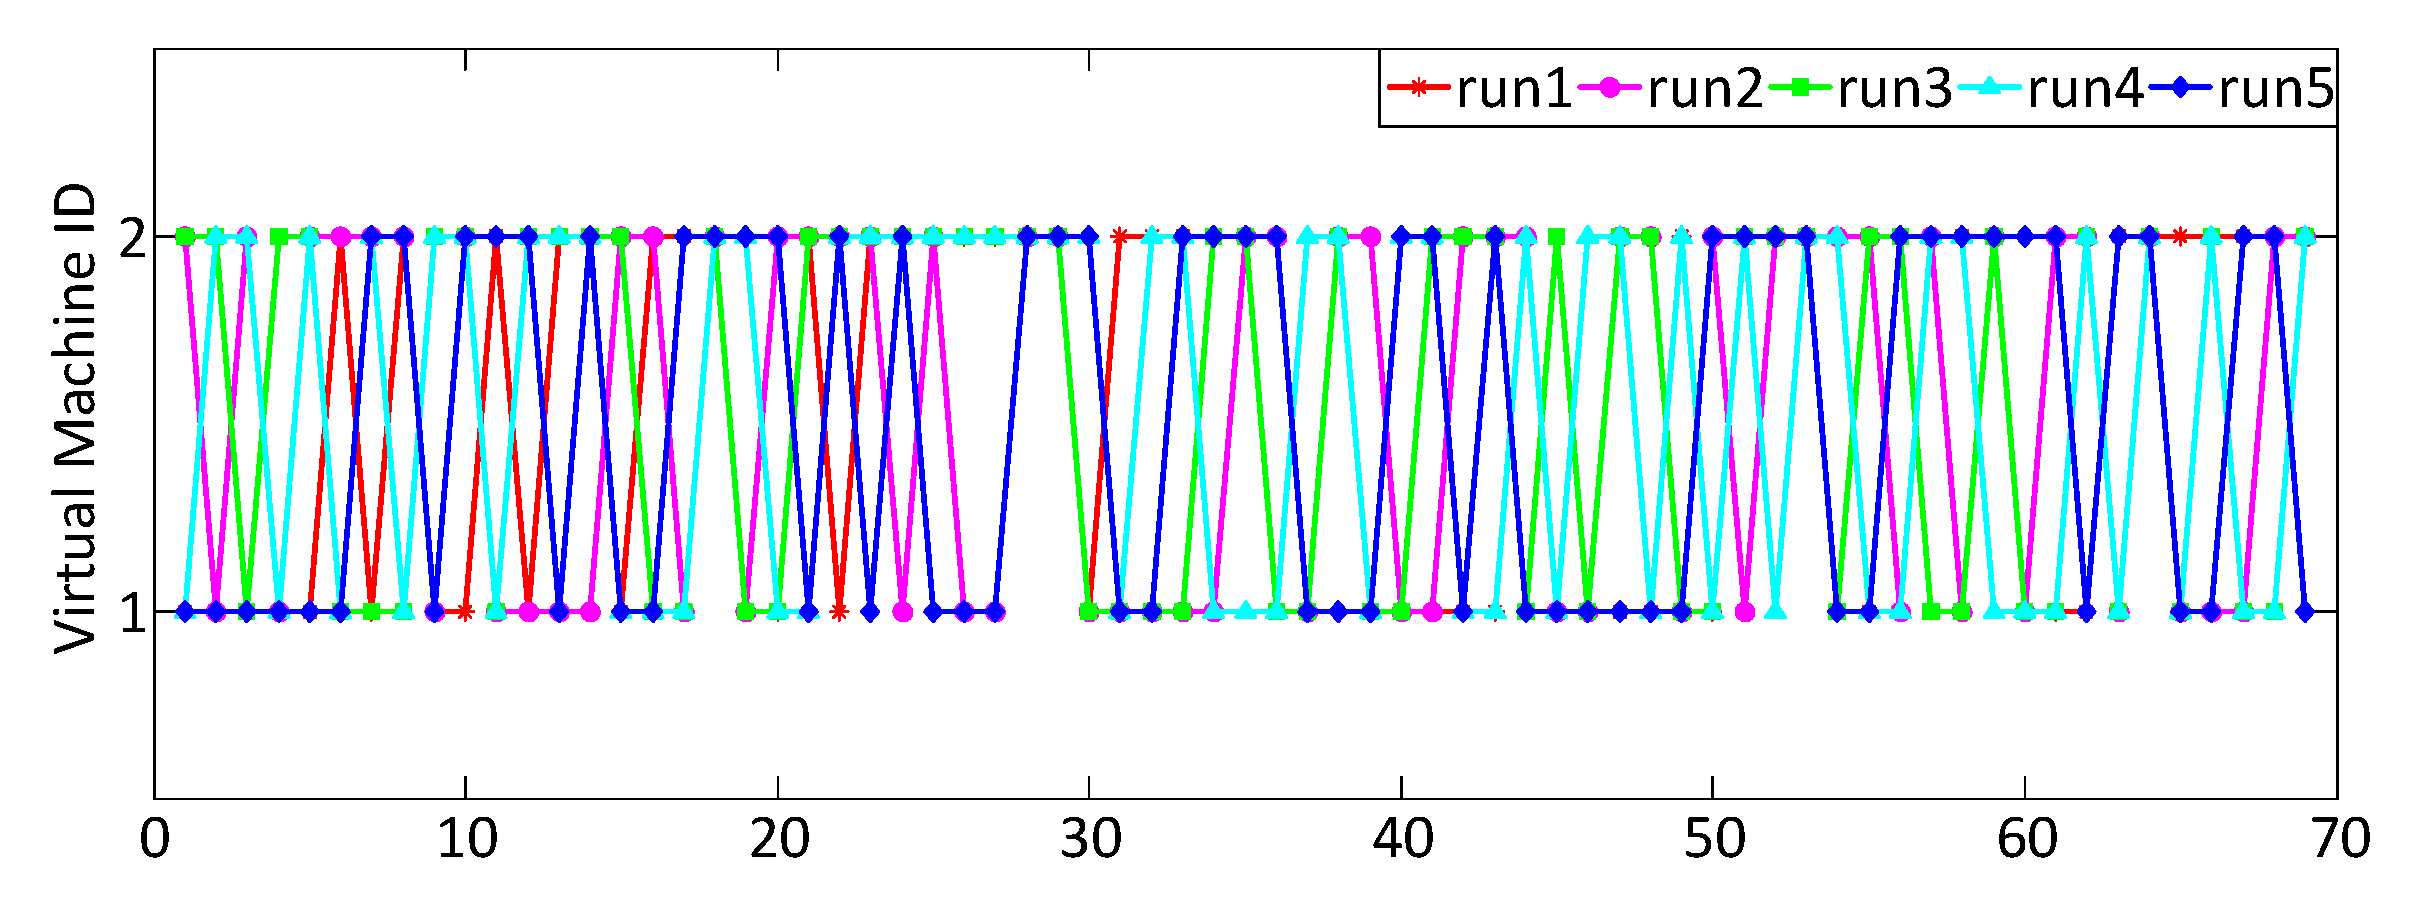
\includegraphics[width=0.8\textwidth]{figure/exec2vm.pdf}
%\caption{Dynamic VM switching during the protected program execution.}\label{fig:Fig.exec2vm}
%\end{figure}

%\begin{figure}[!t]
%\centering
%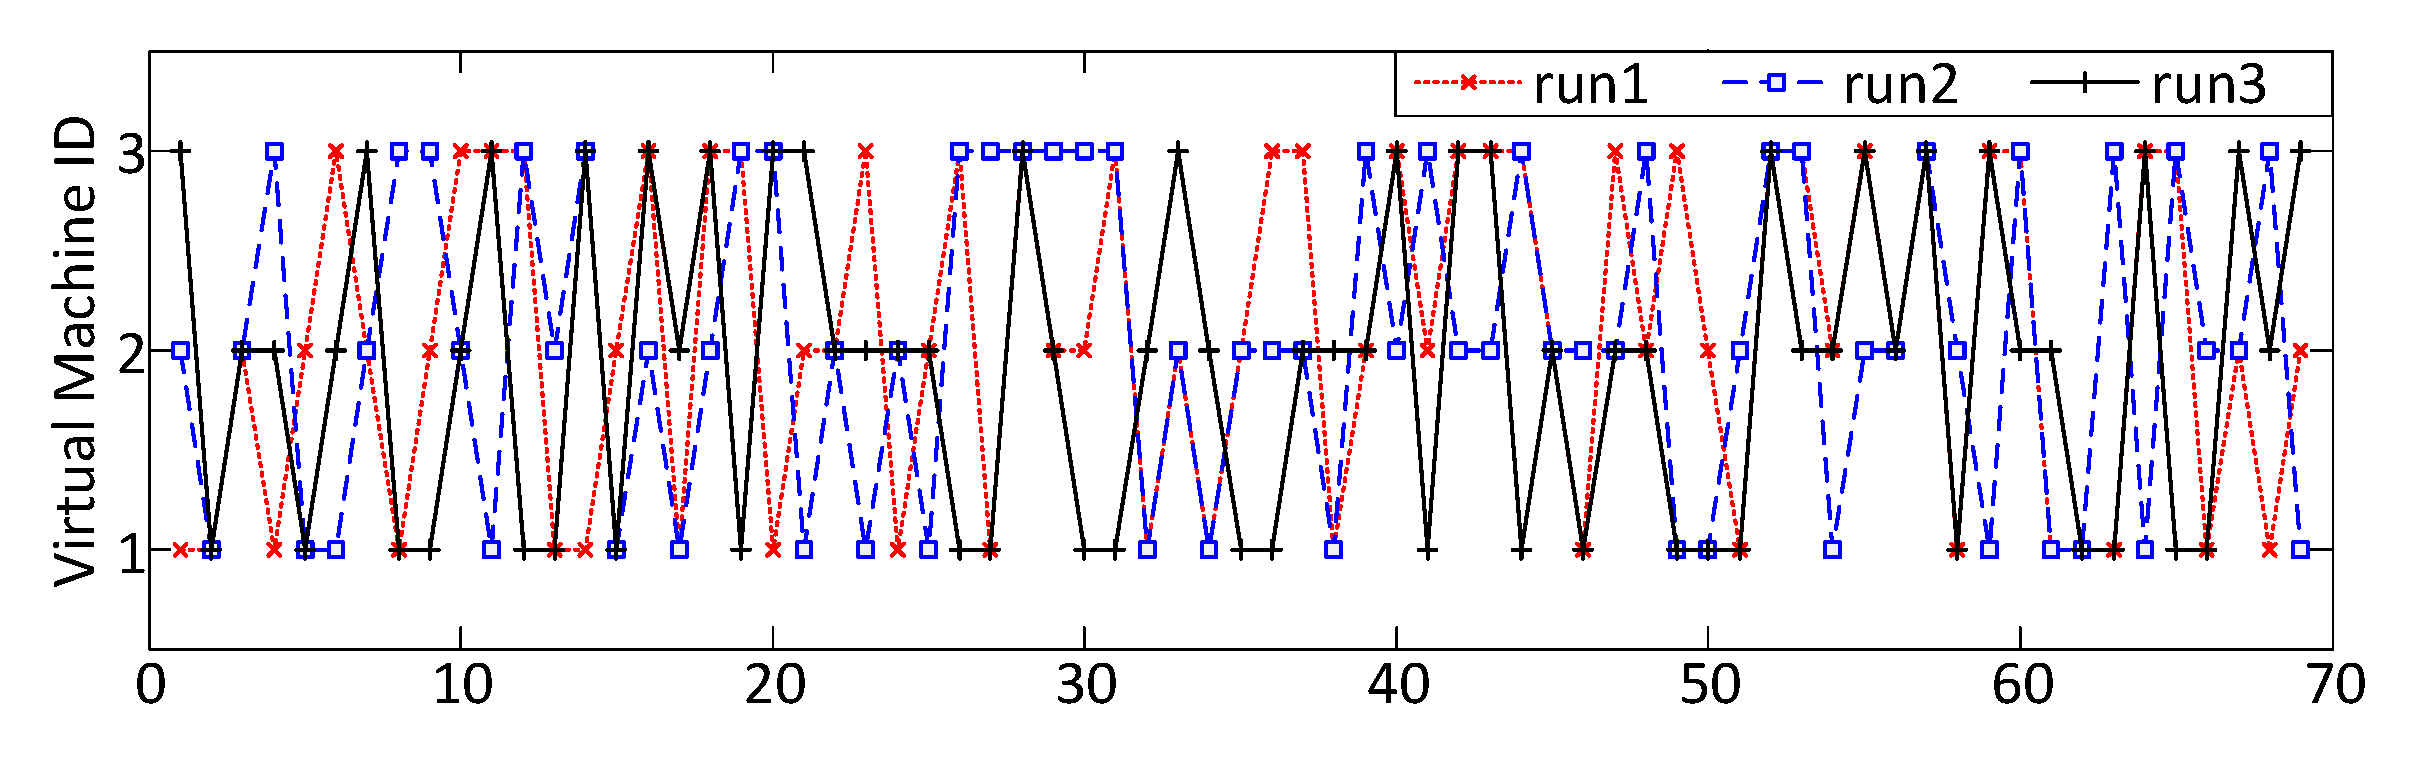
\includegraphics[width=.8\textwidth]{figure/exec3vm.pdf}
%\caption{Dynamic VM switching during the protected program execution.}\label{fig:Fig.exec3vm}
%\end{figure}

%\begin{figure}[!t]
%\centering
%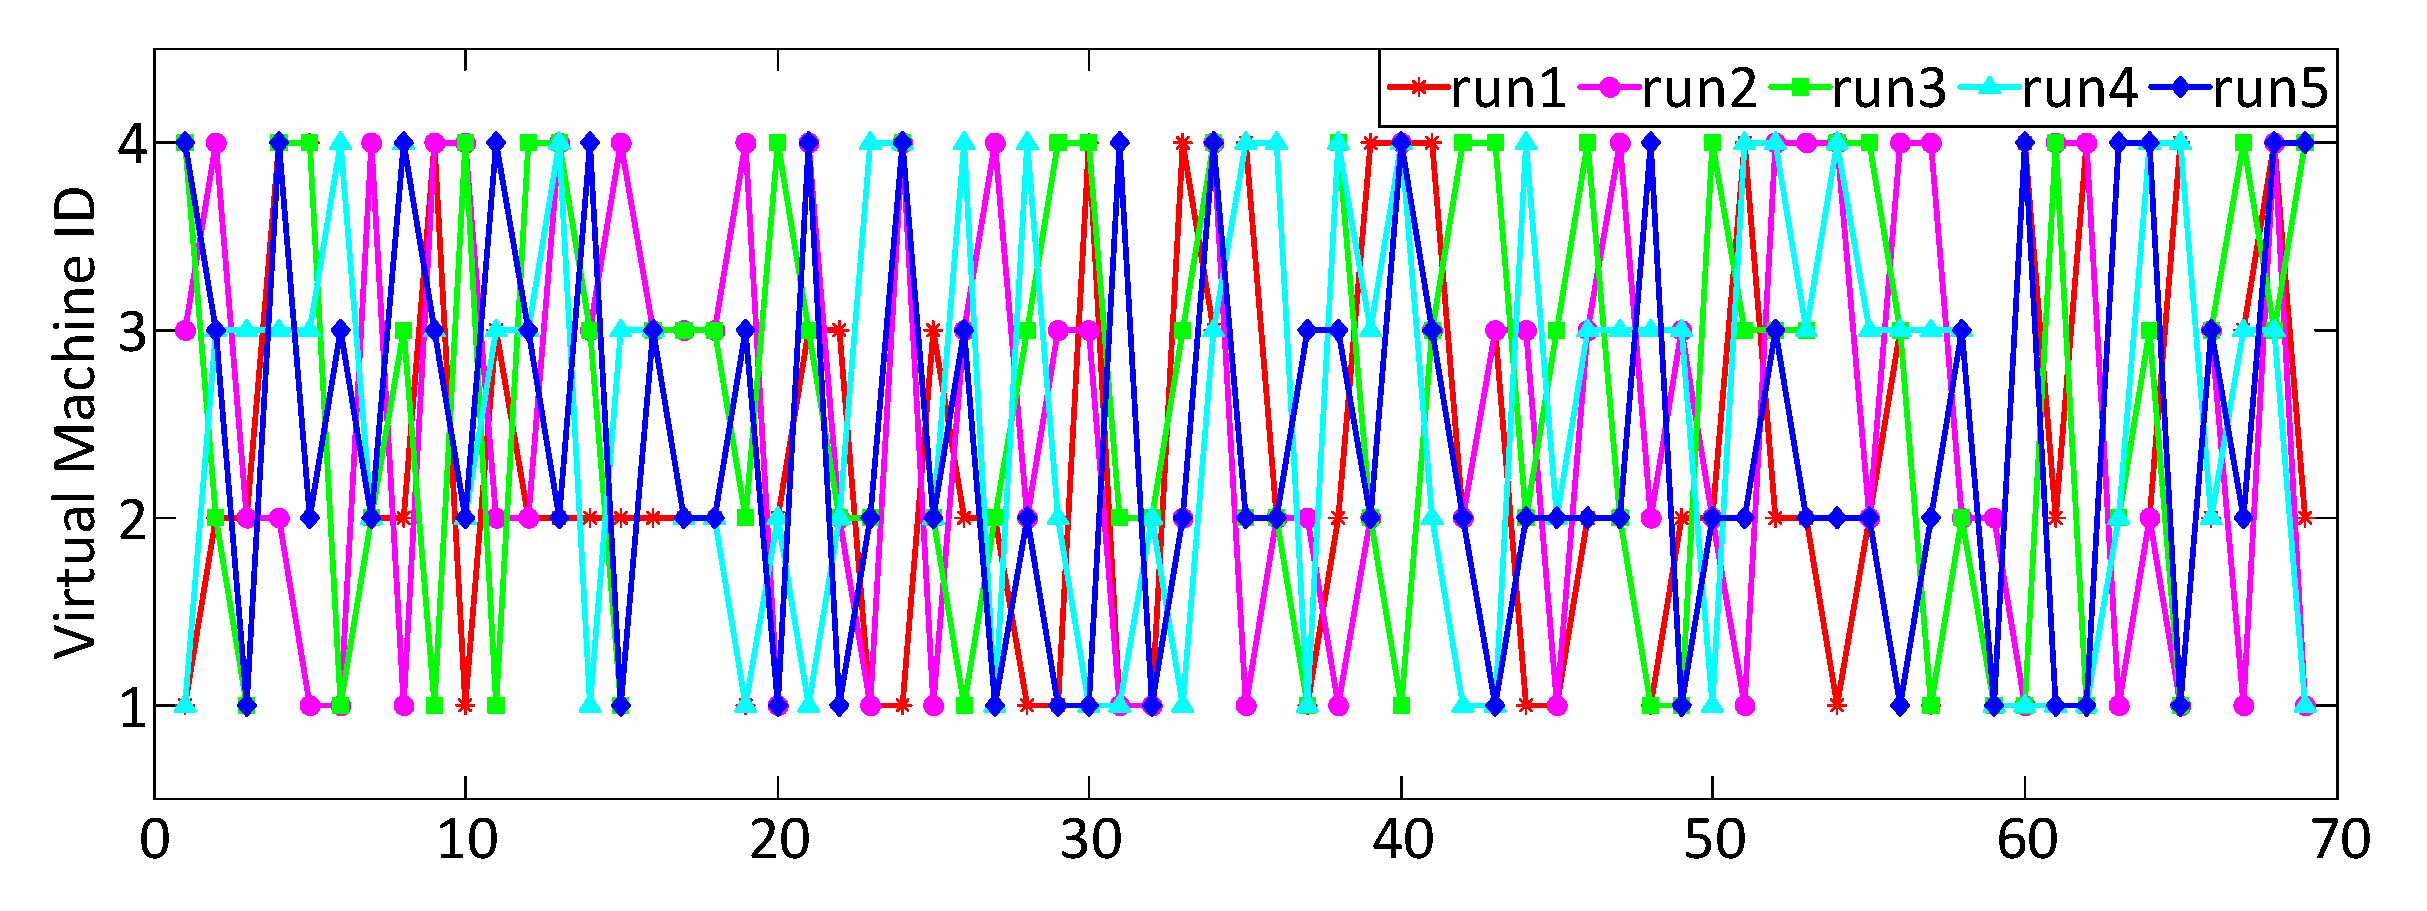
\includegraphics[width=.8\textwidth]{figure/exec4vm.pdf}
%\caption{Dynamic VM switching during the protected program execution.}\label{fig:Fig.exec4vm}
%\end{figure}



\subsection{Comparisons with state-of-the-arts}\label{sec:comparetest}
We also compared \DSVMP against two commercial VM protection systems,
Code Virtualizer (CV)~\cite{2CV} and VMProtect (VMP)~\cite{3Vmprotect}, in terms of code sizes and runtime overhead.
We adopt a custom protection scheme when using the CV to protect the target program,
because such a CV has a moderate temporal and spatial overhead.
In addition, we also adopt the VMP with two kinds of schemes to protect the target program,
\emph{Maximum-protection} and \emph{Maximum-speed}.
For \DSVMP, We used a configuration of 5 VMs, \DSVMP-5VM, in this experiment.

\begin{figure}[t]
\centering
\begin{minipage}[t]{0.49\linewidth}
\centering
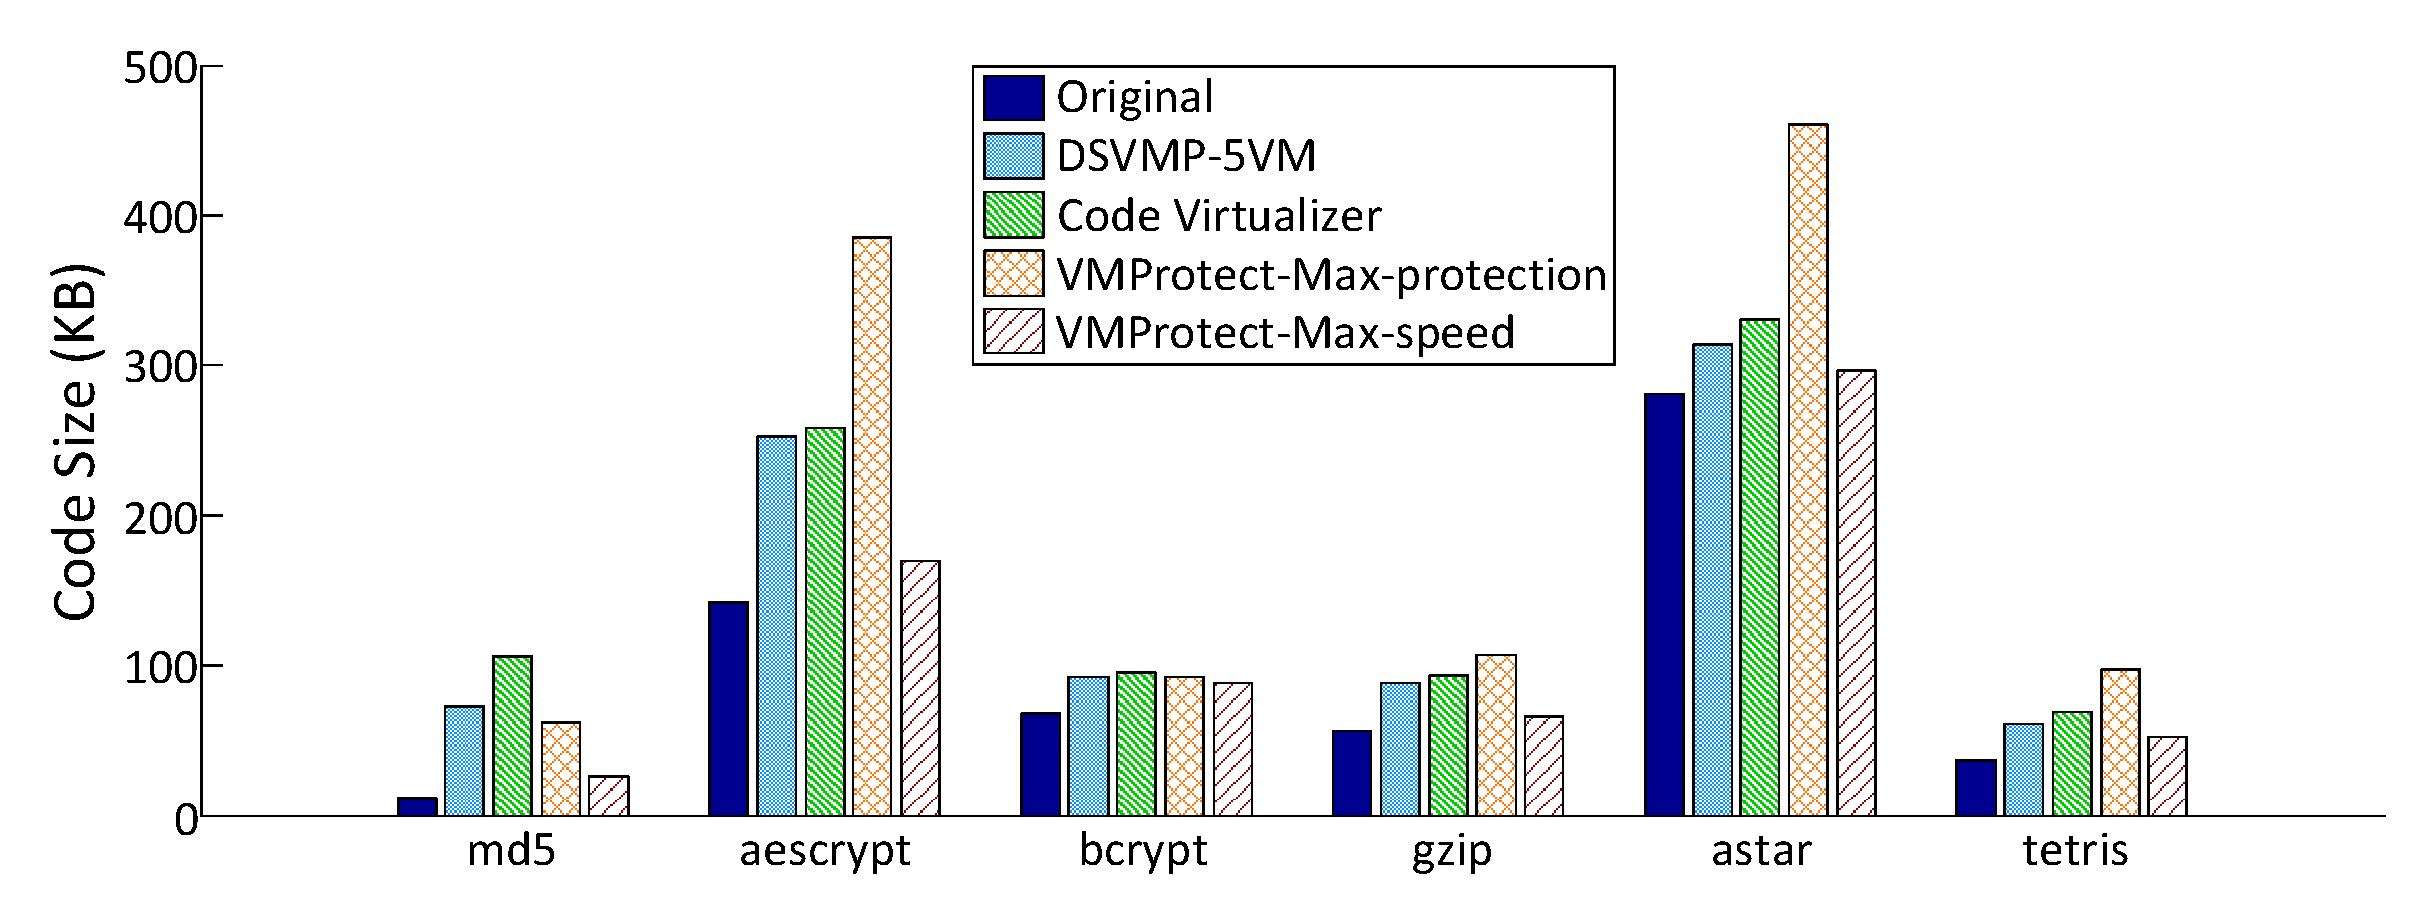
\includegraphics[width=.9\textwidth]{figure/comsize.pdf}
\caption{The comparison of impact on file size with VMProtect and Code Virtualizer.}\label{fig:Fig.com-size}
\end{minipage}
\hspace{0.005\textwidth}
\begin{minipage}[t]{0.49\linewidth}
\centering
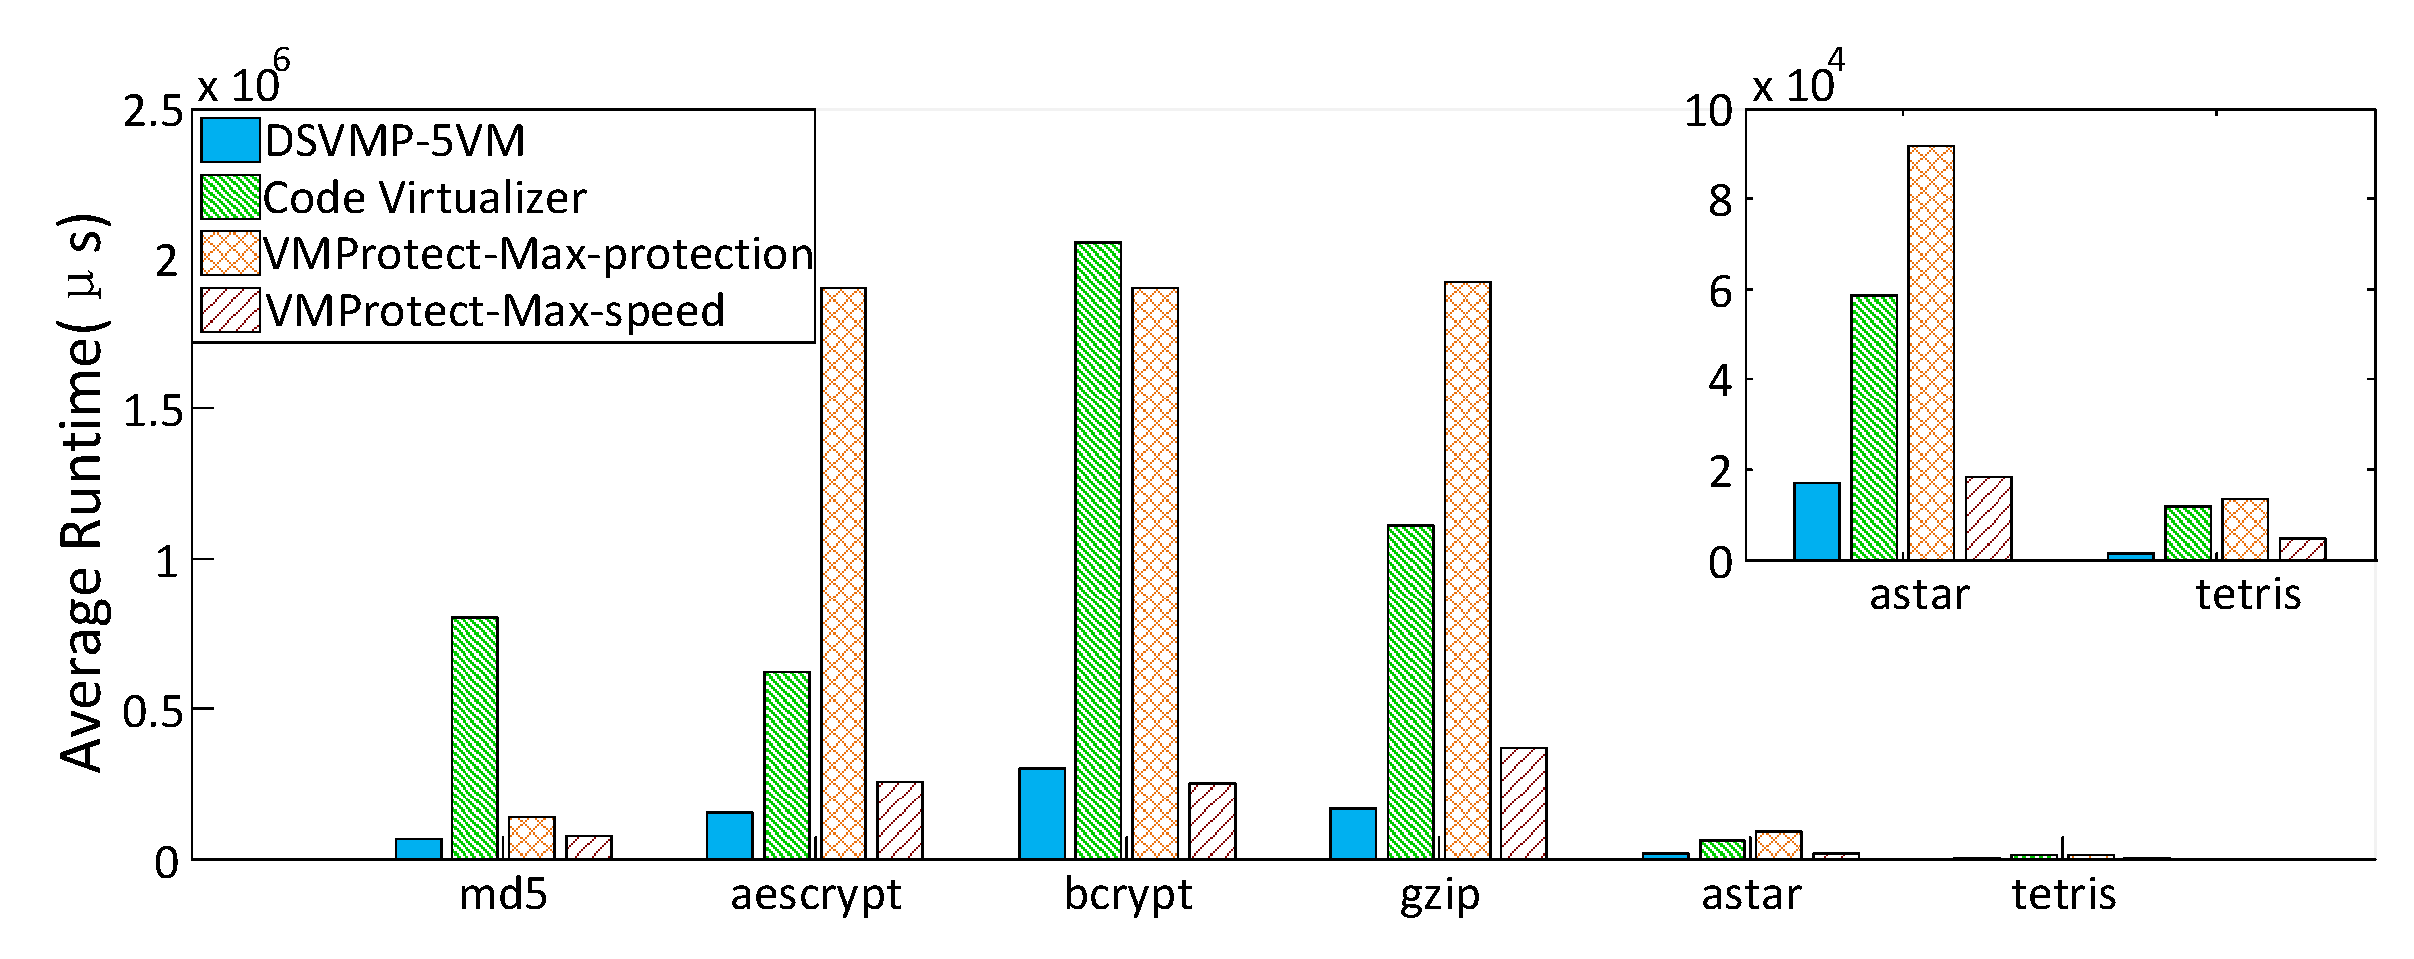
\includegraphics[width=.9\textwidth]{figure/comtime.pdf}
\caption{The comparison of average runtime overhead with VMProtect and Code Virtualizer.}\label{fig:Fig.com-time}
\end{minipage}
\end{figure}


\paragraph*{Code size} Figure \ref{fig:Fig.com-size} shows the impact on code size of several VM-based protection systems.
From the figure we can see that the effects of \DSVMP and commercial VM-based protection systems on code size are similar.
Overall, the expansion of the code size is mainly affected by the size of the protected instructions,
the more the target code brings more spatial overhead.
Among them, the \texttt{aescrypt} has a greater code bloat after protected by VMProtect Maximum-protection,
it may be caused by the complexity of the function \texttt{encrypt-stream()} and the Maximum-protection strategy.


\paragraph*{Runtime overhead} The average runtime overhead of the three schemes are depicted in figure \ref{fig:Fig.com-time},
which shows that the runtime overhead of \DSVMP and VMProtect Maximum-speed
are comparable and smaller than Code Virtualizer and VMProtect Maimum-protection.
Code protected under CV and VMProtect Maimum-protection has the most expensive runtime overhead,
which on average is higher than \DSVMP and VMProtect Maimum-speed.

\paragraph*{Discussion} Through the above analysis and comparison, we argue that the temporal and spatial overhead of our \DSVMP are acceptable.


\section{Related Work}\label{sec:work}
Early work on the binary code protection relies on simple encryption and obfuscation methods,
but they are vulnerable to the sophisticated, diversified attacks developed over the past years.
Traditionally, techniques like junk instructions~\cite{23linn2003obfuscation}, packers~\cite{25Execryptor,26upx},
are used to protect software against attacks based on disassembly and static analysis.
There are also other code protection techniques like code obfuscation~\cite{25wu2010mimimorphism},
control flow and data flow obfuscation~\cite{13liem2008compiler,27ge2005control,27balachandran2014function},
all aim to obfuscate the semantic and logical information of the target program.
In practice, these approaches are often used in combination to provide stronger protection.
\DSVMP also leverages some of the code obfuscation techniques developed in the past for code protection.

There is a growing interest in using code virtualization to protect software from malicious reverse engineering.
Fang \emph{et al.}~\cite{5fang2011multi} proposed a protection scheme based on multi-stage code obfuscation.
Their approach iteratively transforms the critical code region several times with different interpretation methods to improve security.
Yang \emph{et al.}~\cite{6ming2011software} presented a nested virtual machine for code protection.
Using their approach, an adversary would have to fully reverse engineer a layer of the interpreter before moving to the next layer,
which increases the cost of attacks.
Averbuch \emph{et al.}~\cite{27averbuch2011efficient} introduces an encryption and decryption technology
on the basis of VM-based protection. This approach uses the AES algorithm and a customize encryption key
to encrypt the virtual instructions. During runtime, the VM will decrypt the virtual instruction and then
dispatch a handler to interpret the virtual instructions.
Wang \emph{et al.}~\cite{7wang2014tdvmp} proposed a protection scheme to increase the time diversity of protected code regions.
This is achieved by constructing several equivalent but different forms of sub program execution paths,
from which a path will be randomly selected to execute at runtime.

In recent years there are some deobfuscation methods have been proposed.
Coogan \emph{et al.}~\cite{coogan2011deobfuscation} puts forward a behavior based analysis method to analyze the important behavior of code, but it does not pay attention to how to restore the original code structure.
Sharif \emph{et al.}~\cite{sharif2009automatic} used dynamic data-flow and taint analysis to identify data and extract the syntactic and semantic information about the bytecode instructions.
Yadegari \emph{et al.}~\cite{Yadegari2015A}, by tracking the flow of inputs values, and then use semantics-preserving code transformations to simplify the logic of the instructions.
These approach, however, can not restore the structure of the original code completely, and needed taint analysis to get the data flow.

As a departure from prior work, \DSVMP presents a dynamic scheduling structure to improve security for software.
\DSVMP has integrated several novel techniques to increase the diversity and uncertainly of program execution.
These include using a control unit to diversify the execution path of bytecode handlers and using multiple VMs
and dispatchers to randomly schedule instructions from multiple bytecode instruction sets.
Integrating these techniques allows \DSVMP to provide a more diverse program execution structure compared to prior work in the area.
This richer set of diversity can better protect software against code reverse engineering~\cite{20larsen2014sok}.


\section{Conclusions}\label{sec:con}
This paper has presented \DSVMP, a novel VM-based code protection scheme.
\DSVMP uses a dynamic scheduling structure and multiple VMs to increase
diversity of program execution. We have shown that code
segments protected by \DSVMP rarely follow the same execution path across
different runs. The dynamic program execution brought by \DSVMP forces the attacker
to have to use many trail runs to uncover the implementation of the protected code
region. As such, \DSVMP significantly increases the overhead and effort
involved in code reverse engineering. We have evaluated \DSVMP using four
real world applications and compared it to two state-of-the-art VM-based code
protection schemes. Our experimental results show that \DSVMP provide
stronger protection with comparable overhead of runtime and code size.

\section*{Acknowledgment}
This work was partial supported by projects of the National Natural Science Foundation of China
(No. 61373177, No. 61572402, No. 61672427),
the Key Project of Chinese Ministry of Education (No. 211181),
the International Cooperation Foundation of Shaanxi Province, China (No. 2013KW01-02, No. 2015KW-003, No. 2016KW-034),
the China Postdoctoral Science Foundation (grant No. 2012M521797),
the Research Project of Shaanxi Province Department of Education (No. 15JK1734),
the Research Project of NWU, China (No. 14NW28),
and the UK Engineering and Physical Sciences Research Council under grants EP/M01567X/1 (SANDeRs), EP/M015793/1 (DIVIDEND).



%% The Appendices part is started with the command \appendix;
%% appendix sections are then done as normal sections
%\appendix

%\section{Section in Appendix}
%\label{appendix-sec1}

%% References
%%
%% Following citation commands can be used in the body text:
%% Usage of \cite is as follows:
%%   \cite{key}         ==>>  [#]
%%   \cite[chap. 2]{key} ==>> [#, chap. 2]
%%

%% References with bibTeX database:

\bibliographystyle{elsarticle-num}
% \bibliographystyle{elsarticle-harv}
% \bibliographystyle{elsarticle-num-names}
% \bibliographystyle{model1a-num-names}
% \bibliographystyle{model1b-num-names}
% \bibliographystyle{model1c-num-names}
% \bibliographystyle{model1-num-names}
% \bibliographystyle{model2-names}
% \bibliographystyle{model3a-num-names}
% \bibliographystyle{model3-num-names}
% \bibliographystyle{model4-names}
% \bibliographystyle{model5-names}
% \bibliographystyle{model6-num-names}

\bibliography{reference}


\end{document}

%%
%% End of file `elsarticle-template-num.tex'.
